\documentclass[utf8]{article}
\usepackage{amsmath,amssymb}
\usepackage{graphicx}
\usepackage{fullpage}
\usepackage{setspace}
\usepackage{verbatim}

\usepackage{algorithm}
\usepackage{algorithm}
\usepackage{algorithmicx}
\usepackage{algpseudocode}
\usepackage{amsmath}
\usepackage[top=2cm, bottom=2cm, left=2cm, right=2cm]{geometry}

\onehalfspacing

\title{\bf\huge Ray Tracing Renderer}
\author{Mei Yixuan}
\date{\today}

\begin{document}
\maketitle

\section{Introduction}
This document describes the design of a simple ray tracing renderer, along with some sample scenes rendered using it. I finished it as course project for Advanced Computer Graphics, given by Prof. Shimming Hu in Tsinghua University.

Complete code for this renderer can be found in https://github.com/AntonyMei/RayTracingRender, along with all external libraries and resources. This code is designed for this course project only and implies no warranty, use at your own risk. All code follow Apache License 2.0, except those external libraries and resources.

\section{Results}
This section shows some of the demo scenes rendered using this renderer. All scenes are rendered under 3840 * 2160 (or 3840 * 3840 if aspect ratio is 1) with more than 1000 samples per pixel and tracing depth 50.

\subsection{Hollow Glass Ball}
\begin{figure}[H]
	\centering
	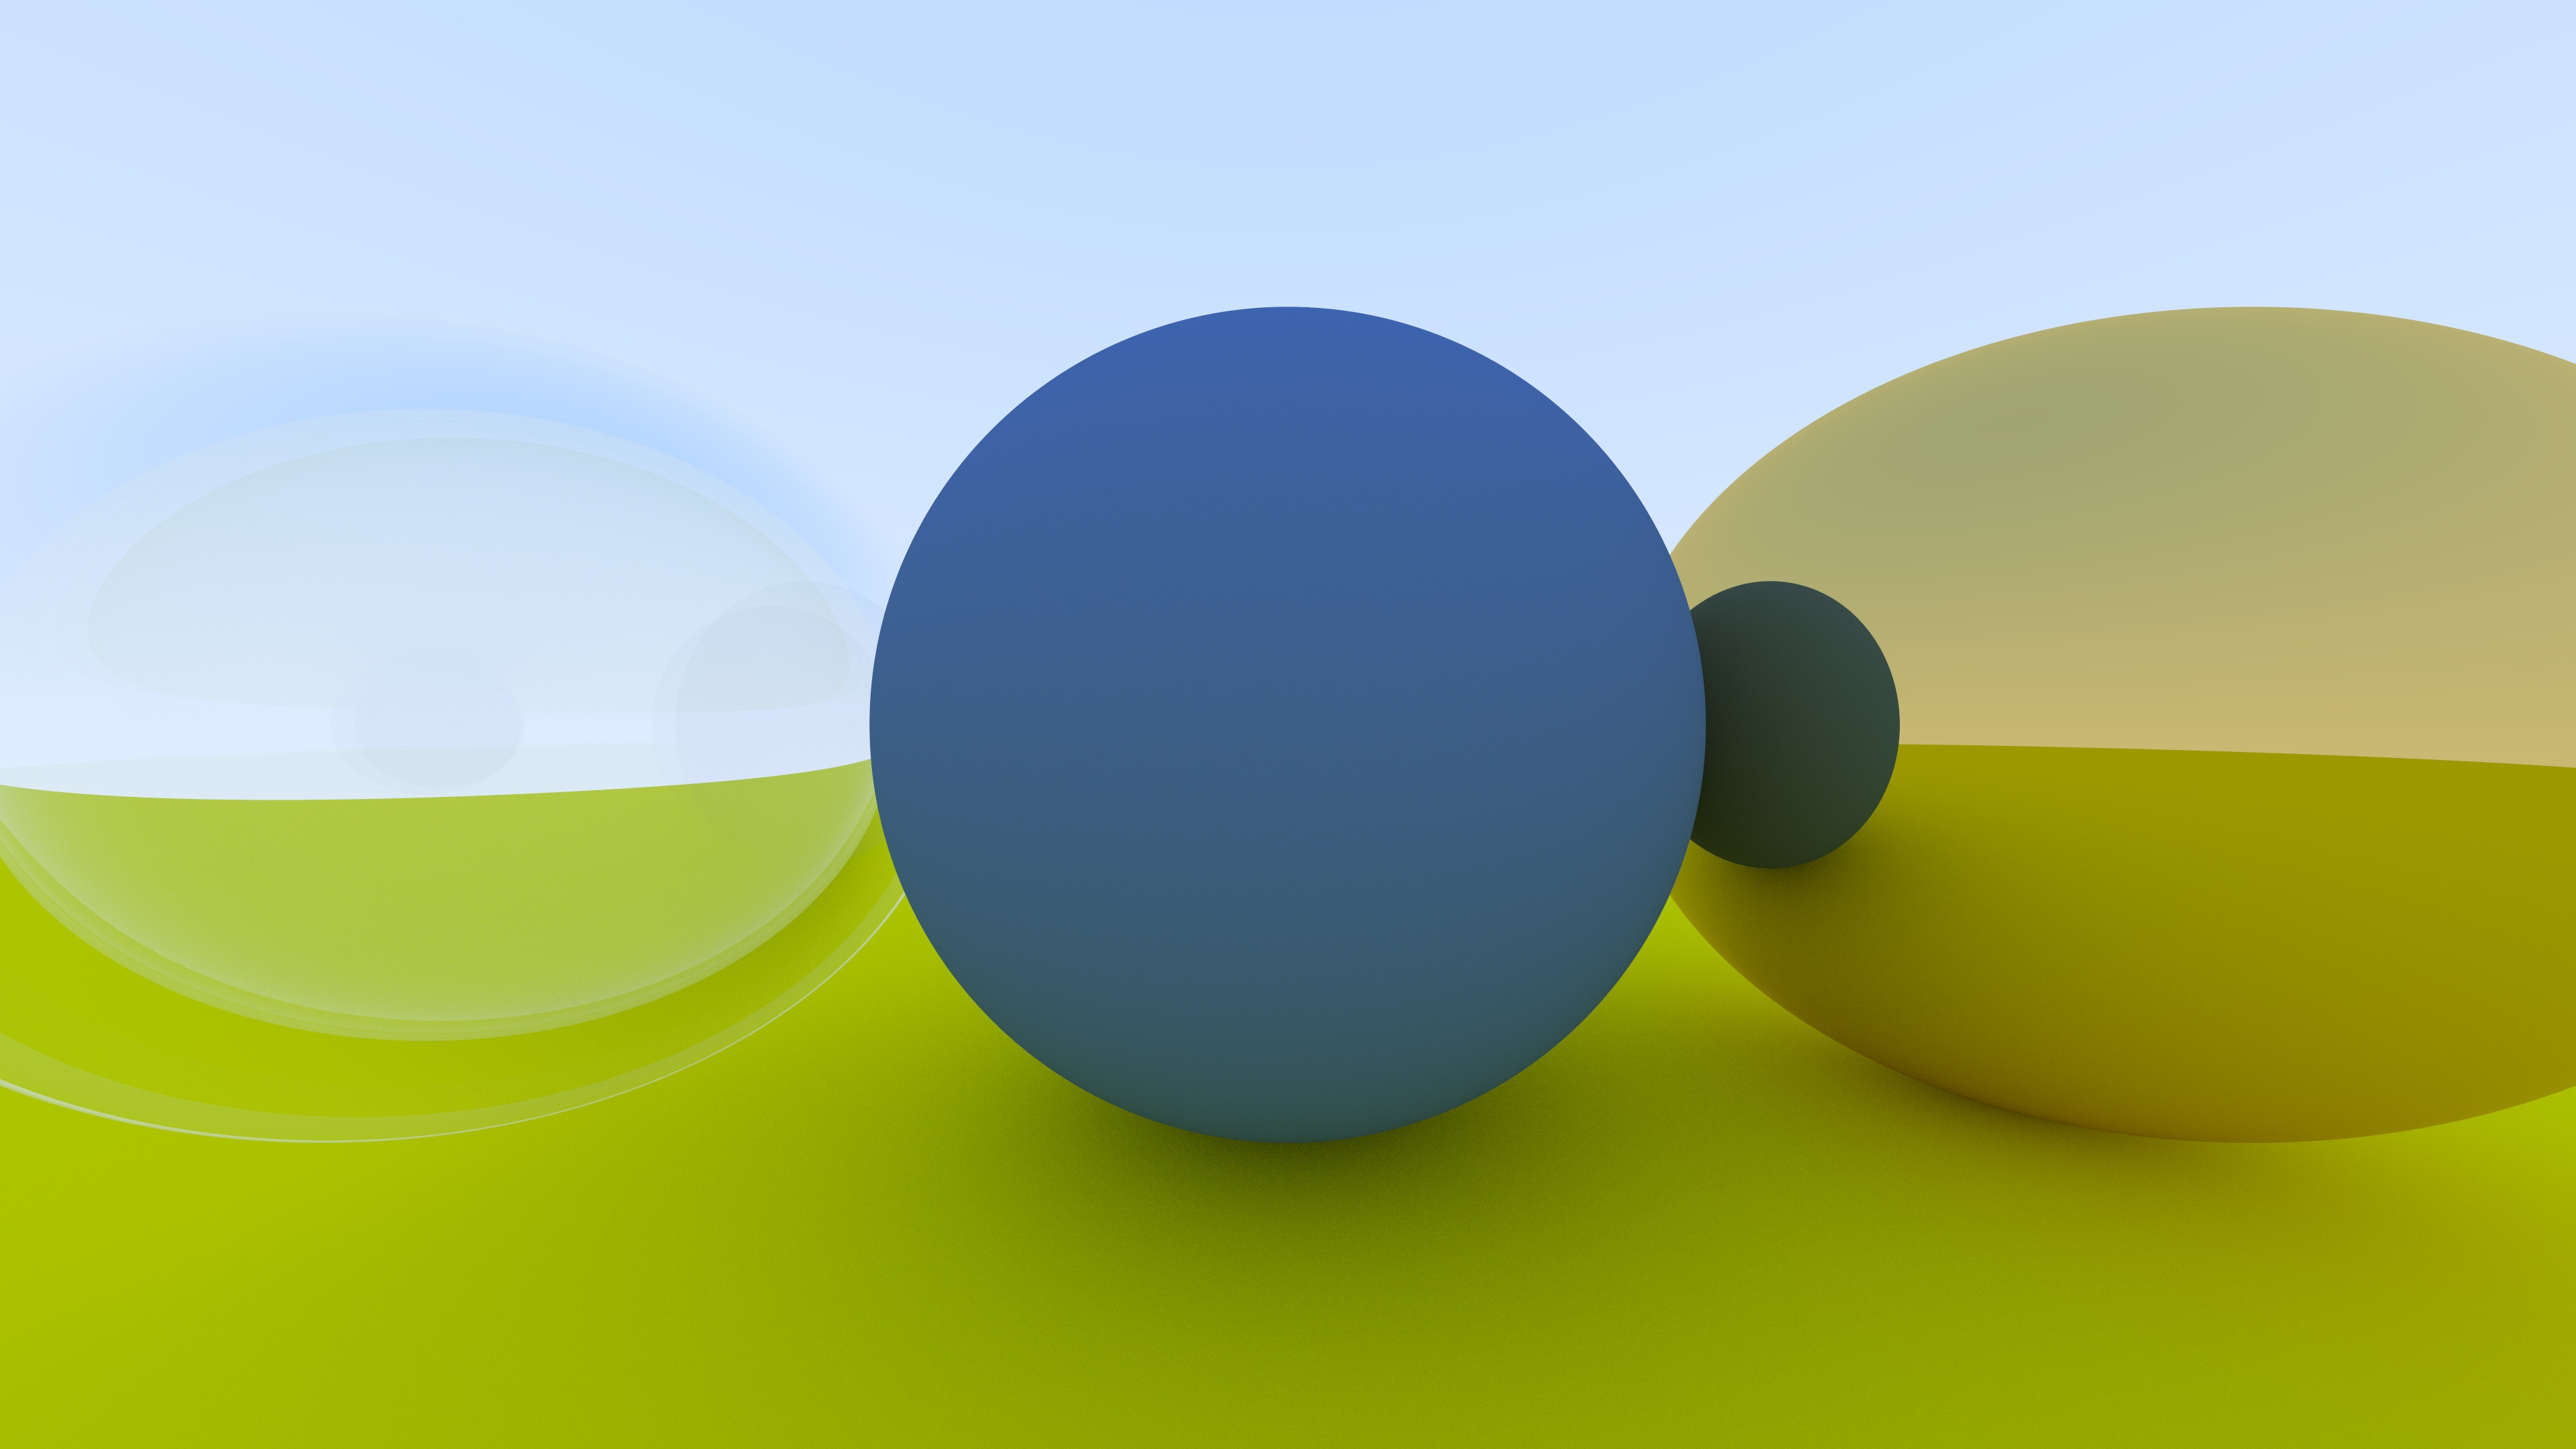
\includegraphics[width=0.7\linewidth]{../_results/hollow_glass_ball}
	\caption{Hollow Glass Ball}
	\label{fig:hollowglassball}
\end{figure}
This scene shows the usage of Lambertian (pure diffuse), Metallic (pure reflection) and Dielectric (refraction) material.

\subsection{Hollow Glass Ball Small FOV}
\begin{figure}[H]
	\centering
	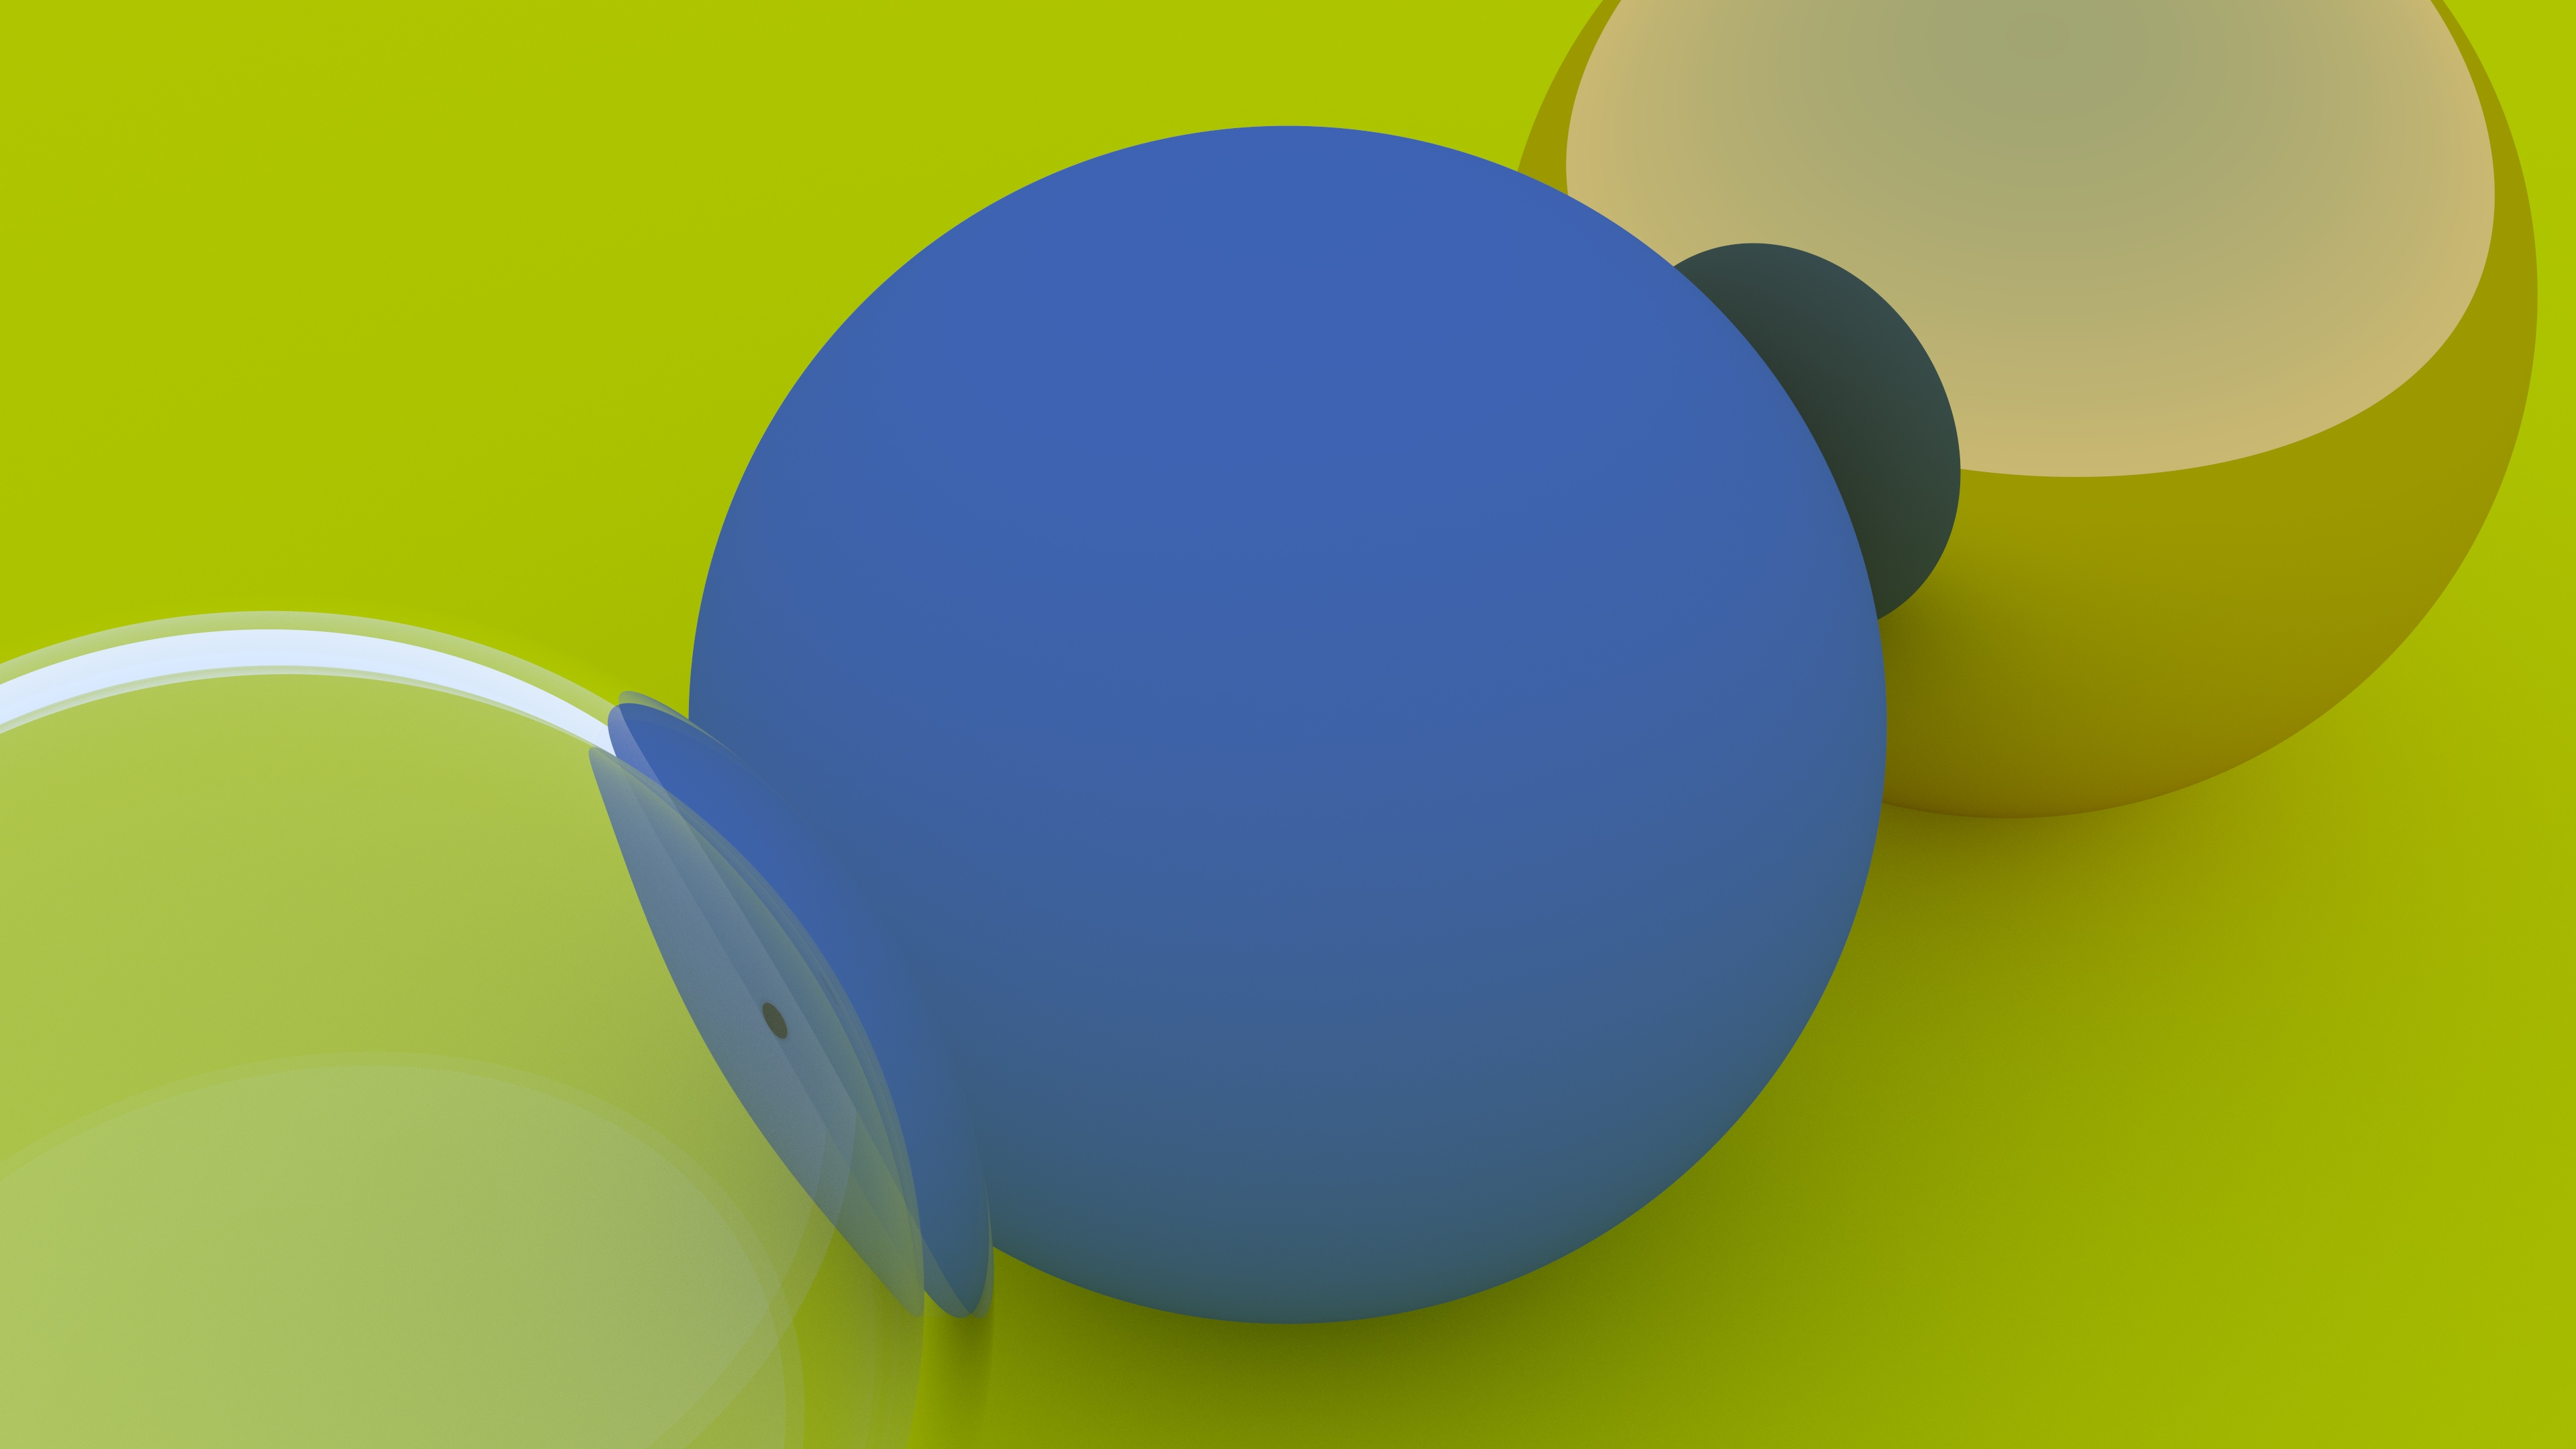
\includegraphics[width=0.7\linewidth]{../_results/hollow_glass_ball_small_fov}
	\caption{Hollow Glass Ball Small FOV}
	\label{fig:hollowglassballsmallfov}
\end{figure}
This scene is identical to the last one, but with smaller camera FOV. Note that edge of the dielectric ball has reflection rather than refraction, which is physically accurate.

\subsection{Hollow Glass Ball Off Focus}
\begin{figure}[H]
	\centering
	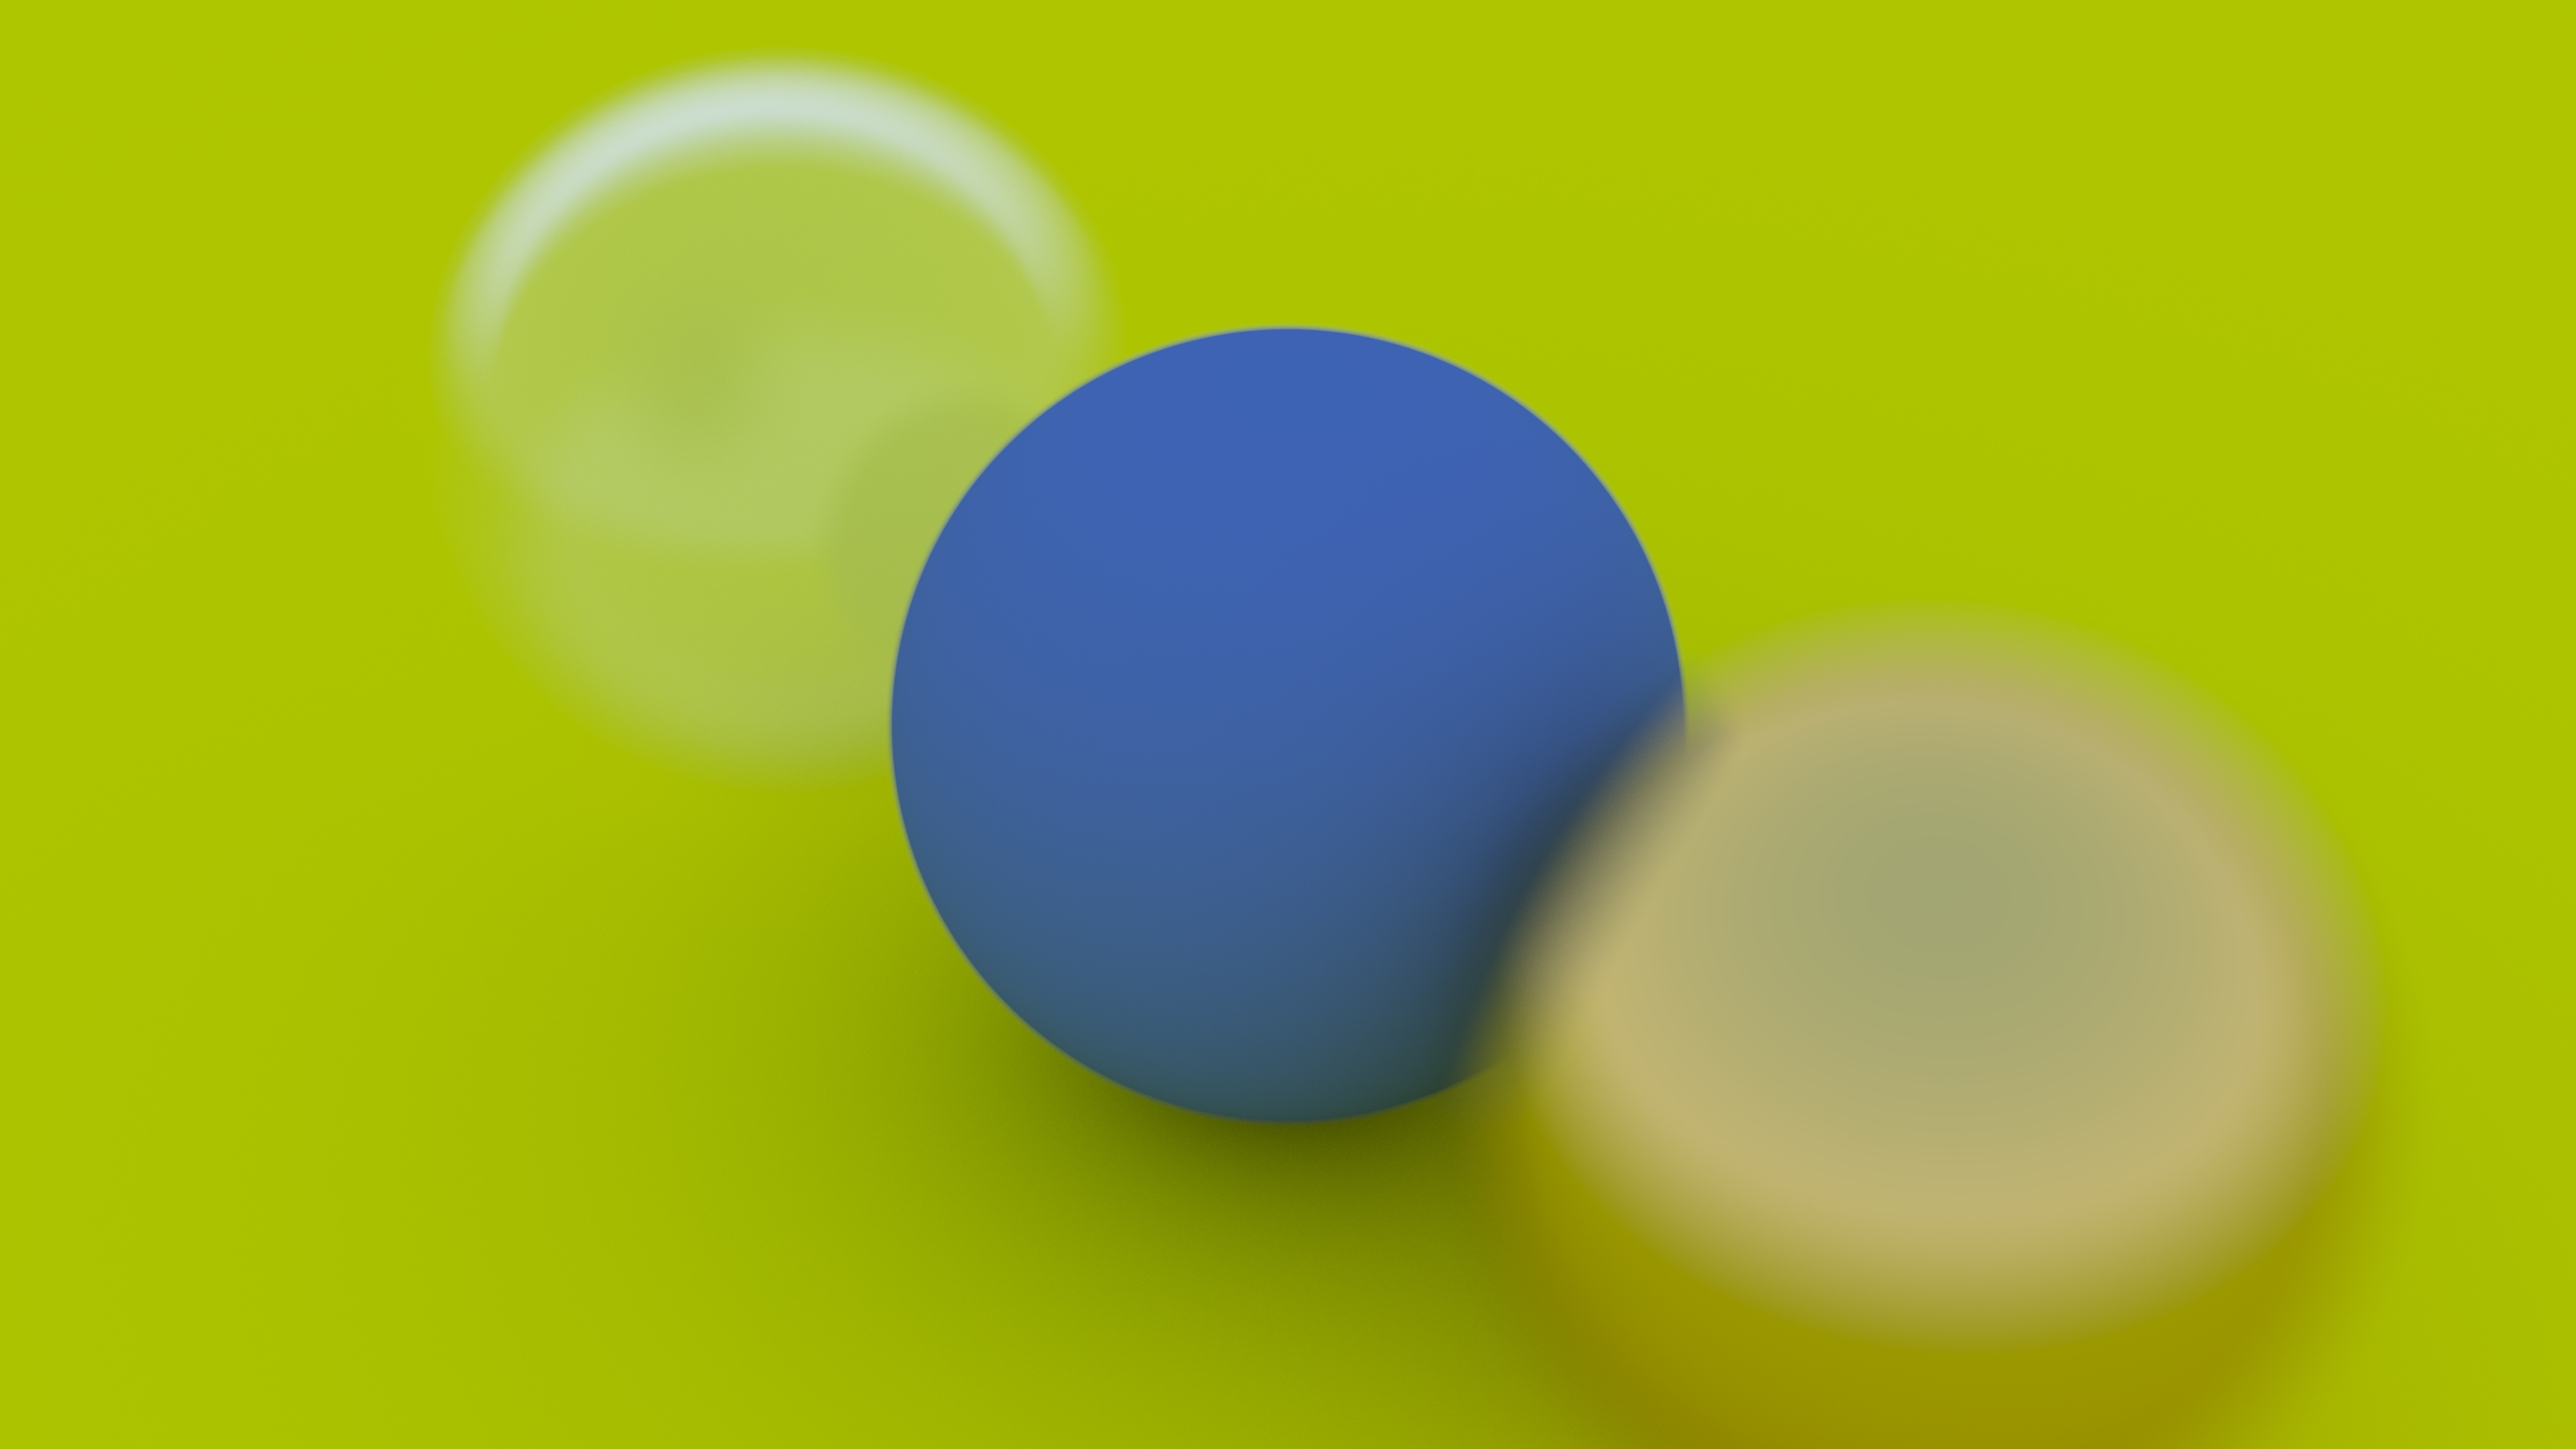
\includegraphics[width=0.7\linewidth]{../_results/hollow_glass_ball_off_focus}
	\caption{Hollow Glass Ball Off Focus}
	\label{fig:hollowglassballofffocus}
\end{figure}
This scene shows off-focus blur effect.

\subsection{Many Balls}
\begin{figure}[H]
	\centering
	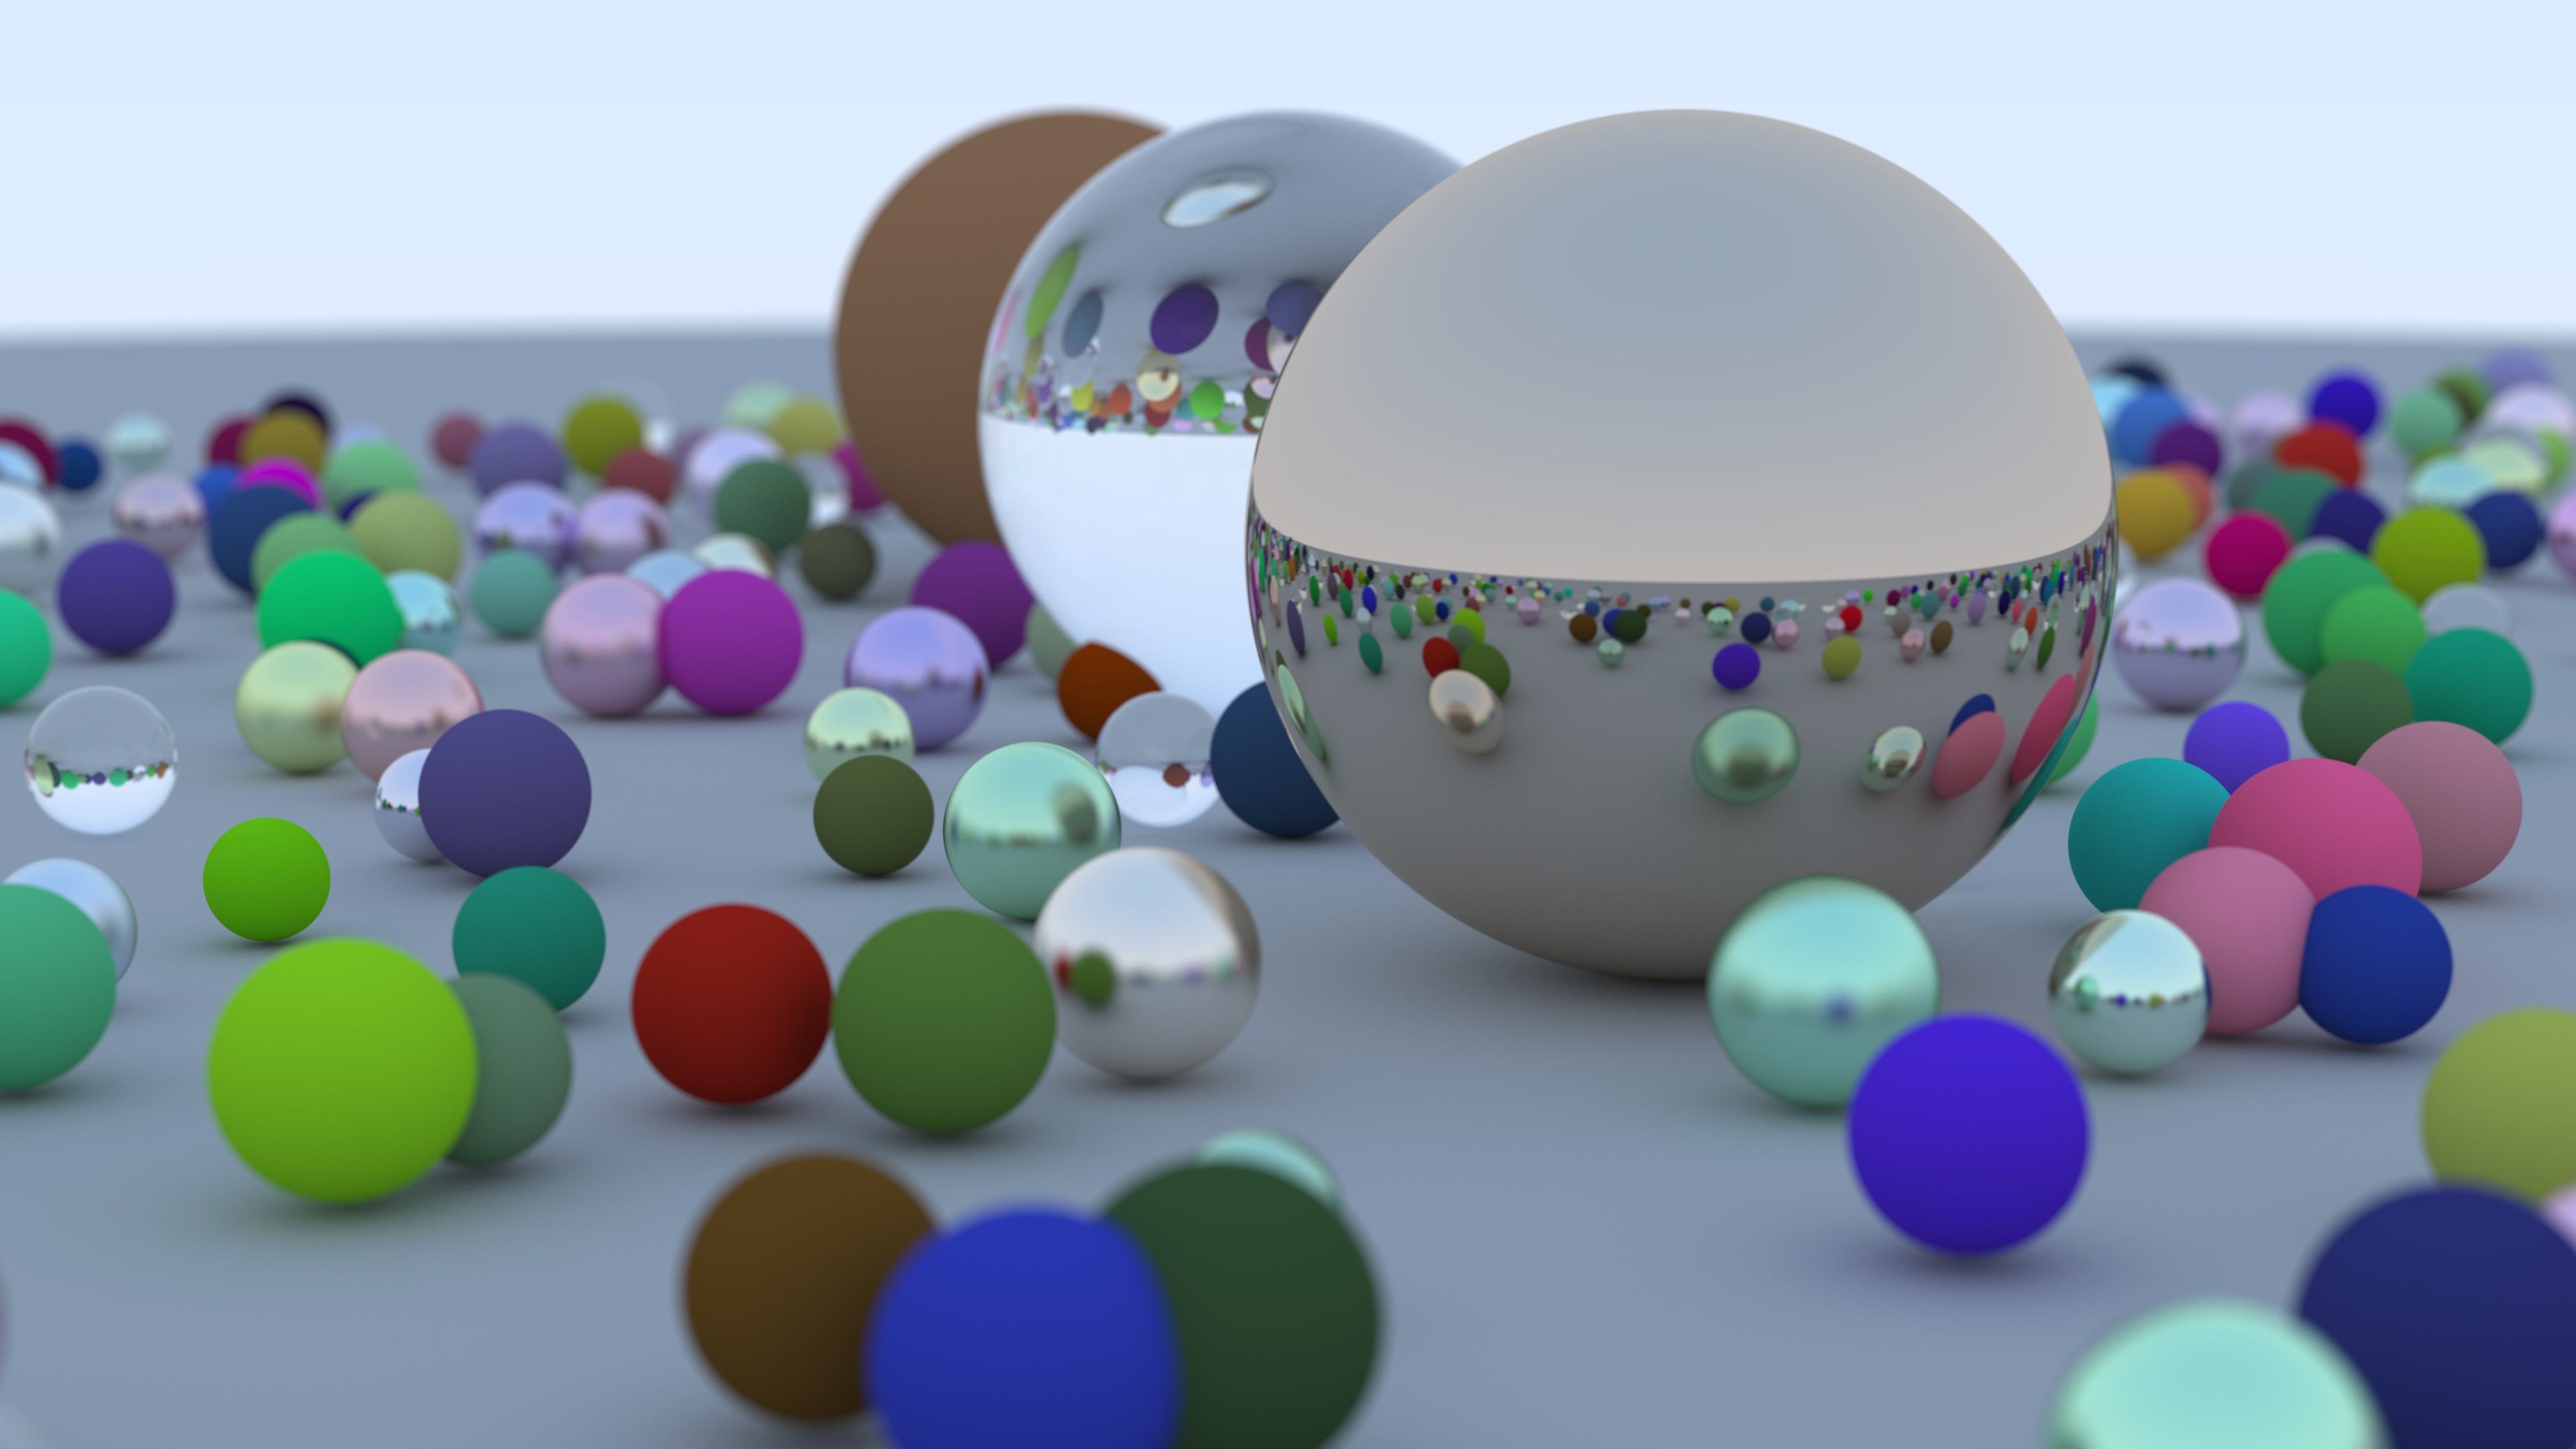
\includegraphics[width=0.7\linewidth]{../_results/many_balls}
	\caption{Many Balls}
	\label{fig:manyballs}
\end{figure}
This scene contain many balls. Note that metallic material can use fuzziness to simulate imperfect reflection.

\subsection{Motion Blur}
\begin{figure}[H]
	\centering
	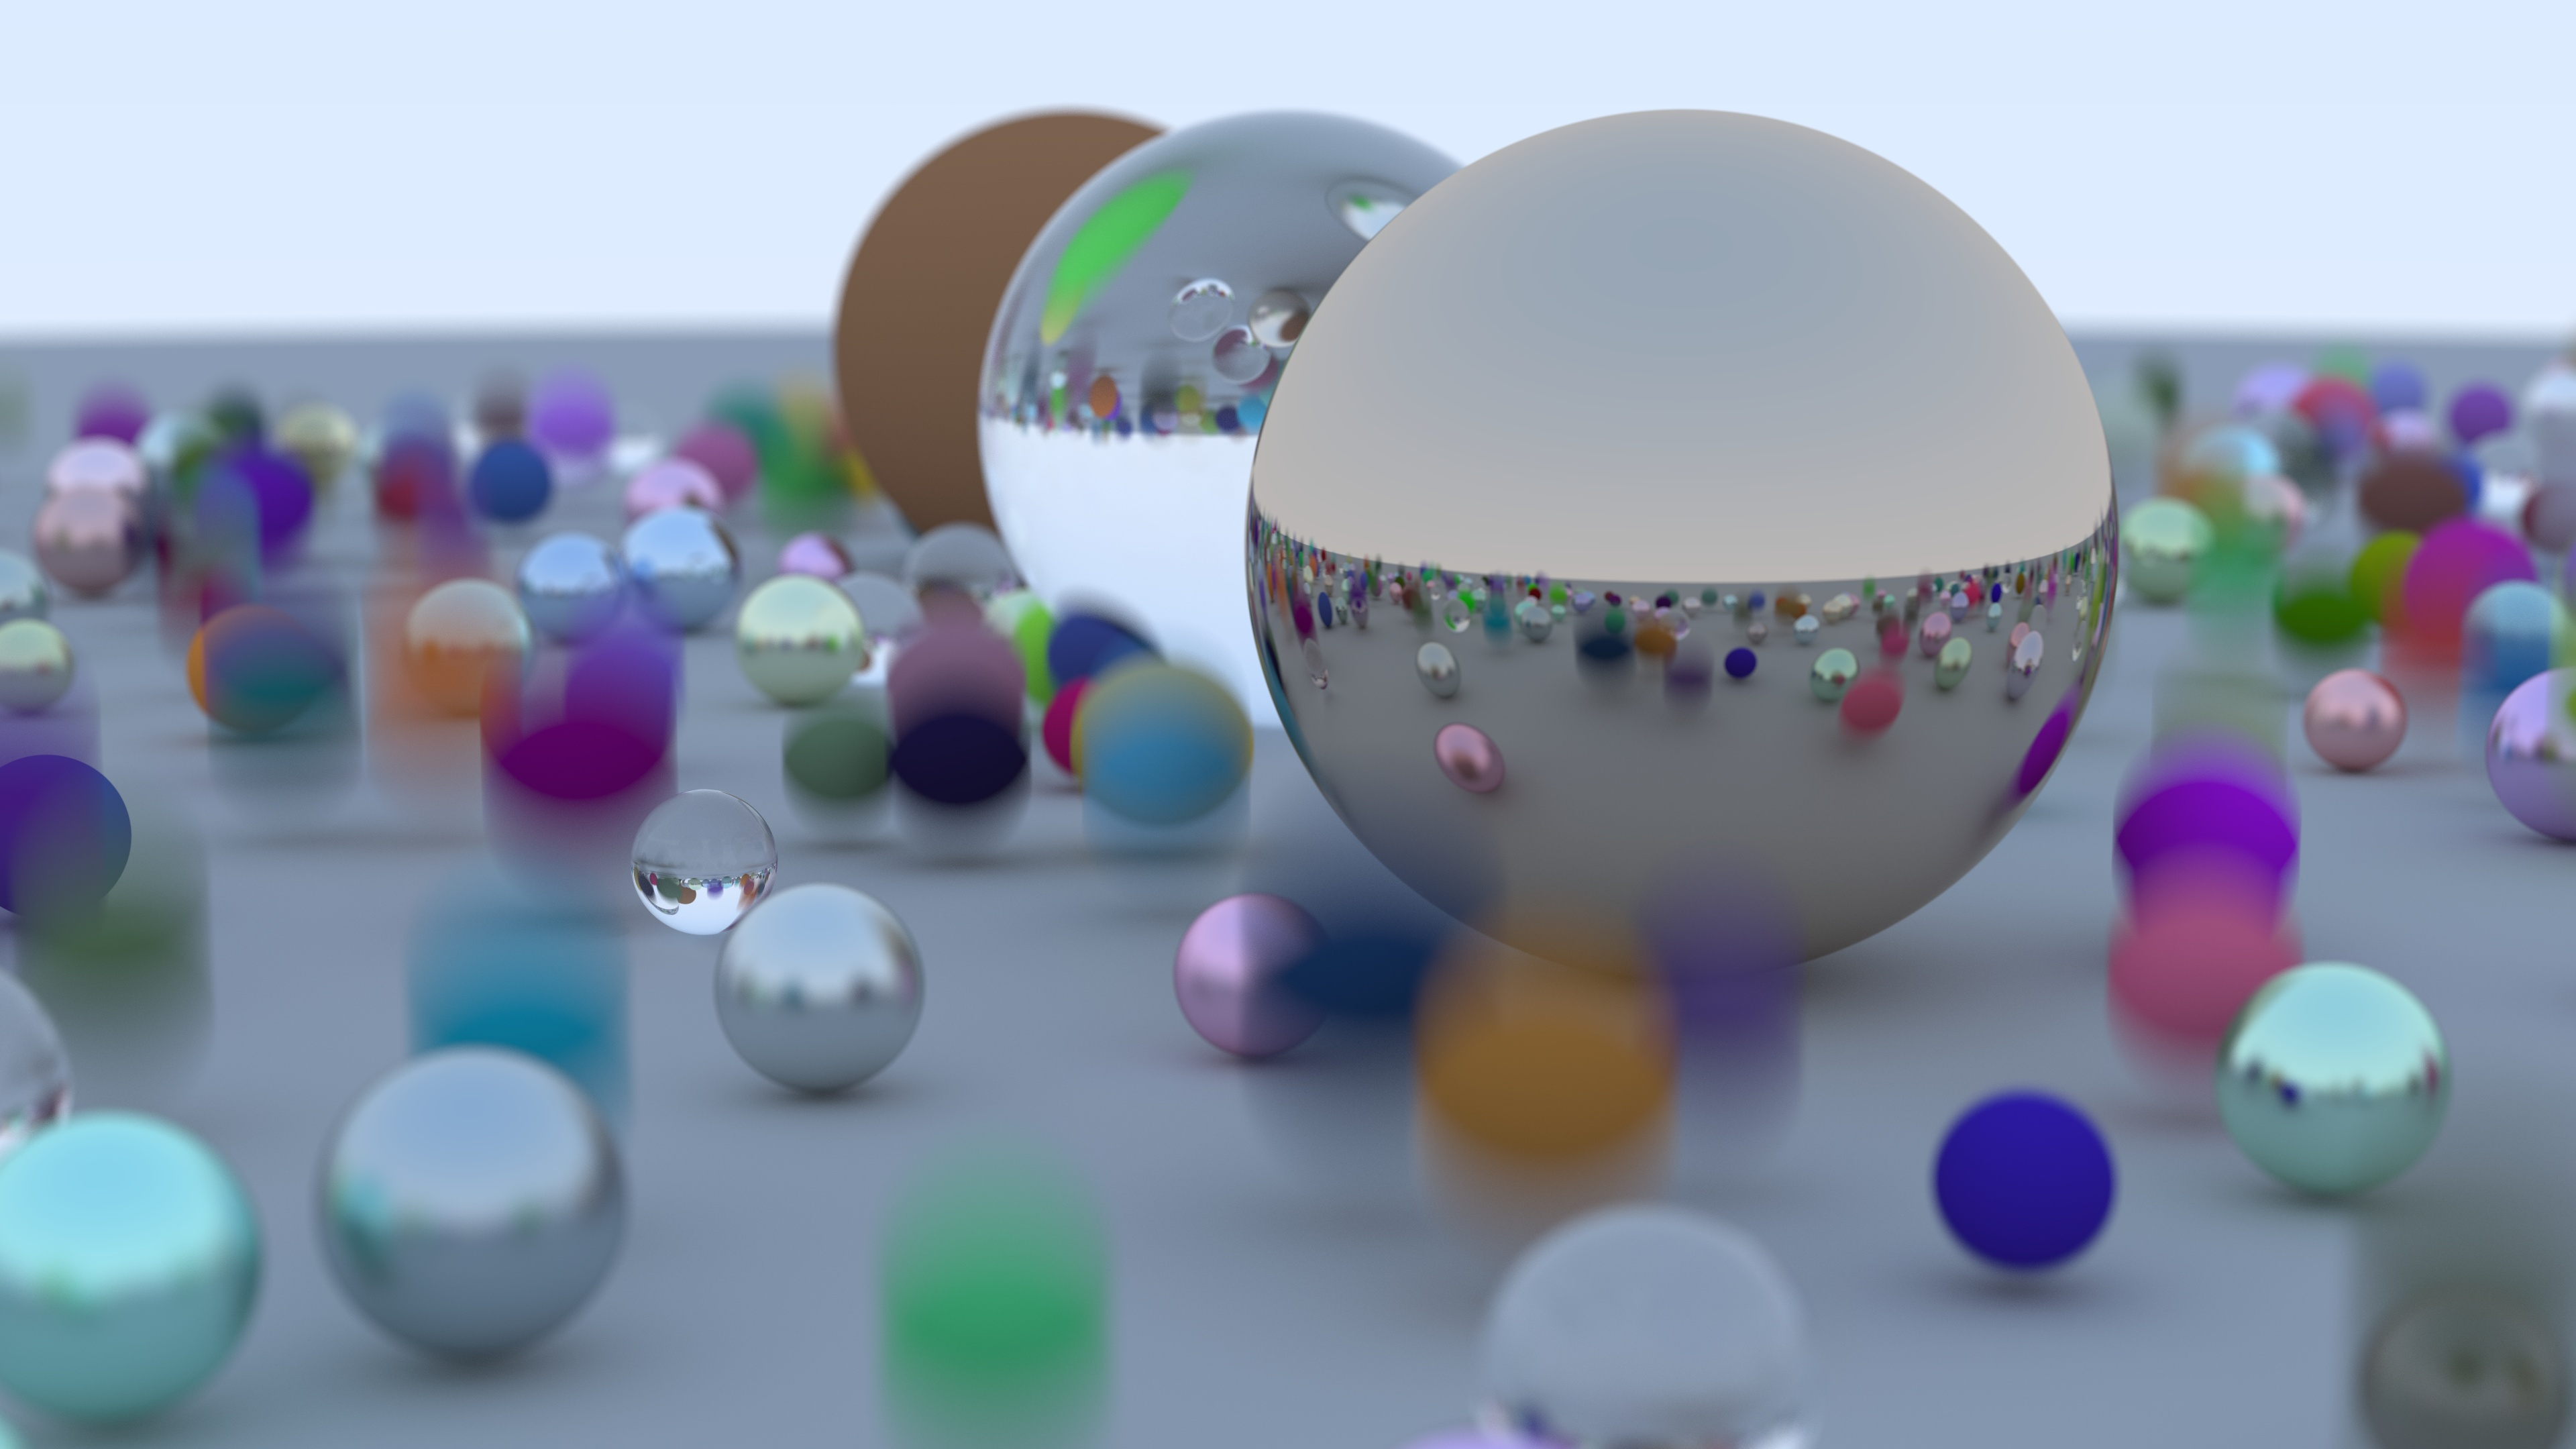
\includegraphics[width=0.7\linewidth]{../_results/motion_blur}
	\caption{Motion Blur}
	\label{fig:motionblur}
\end{figure}
This scene shows motion blur effect.

\subsection{Motion Blur Checker}
\begin{figure}[H]
	\centering
	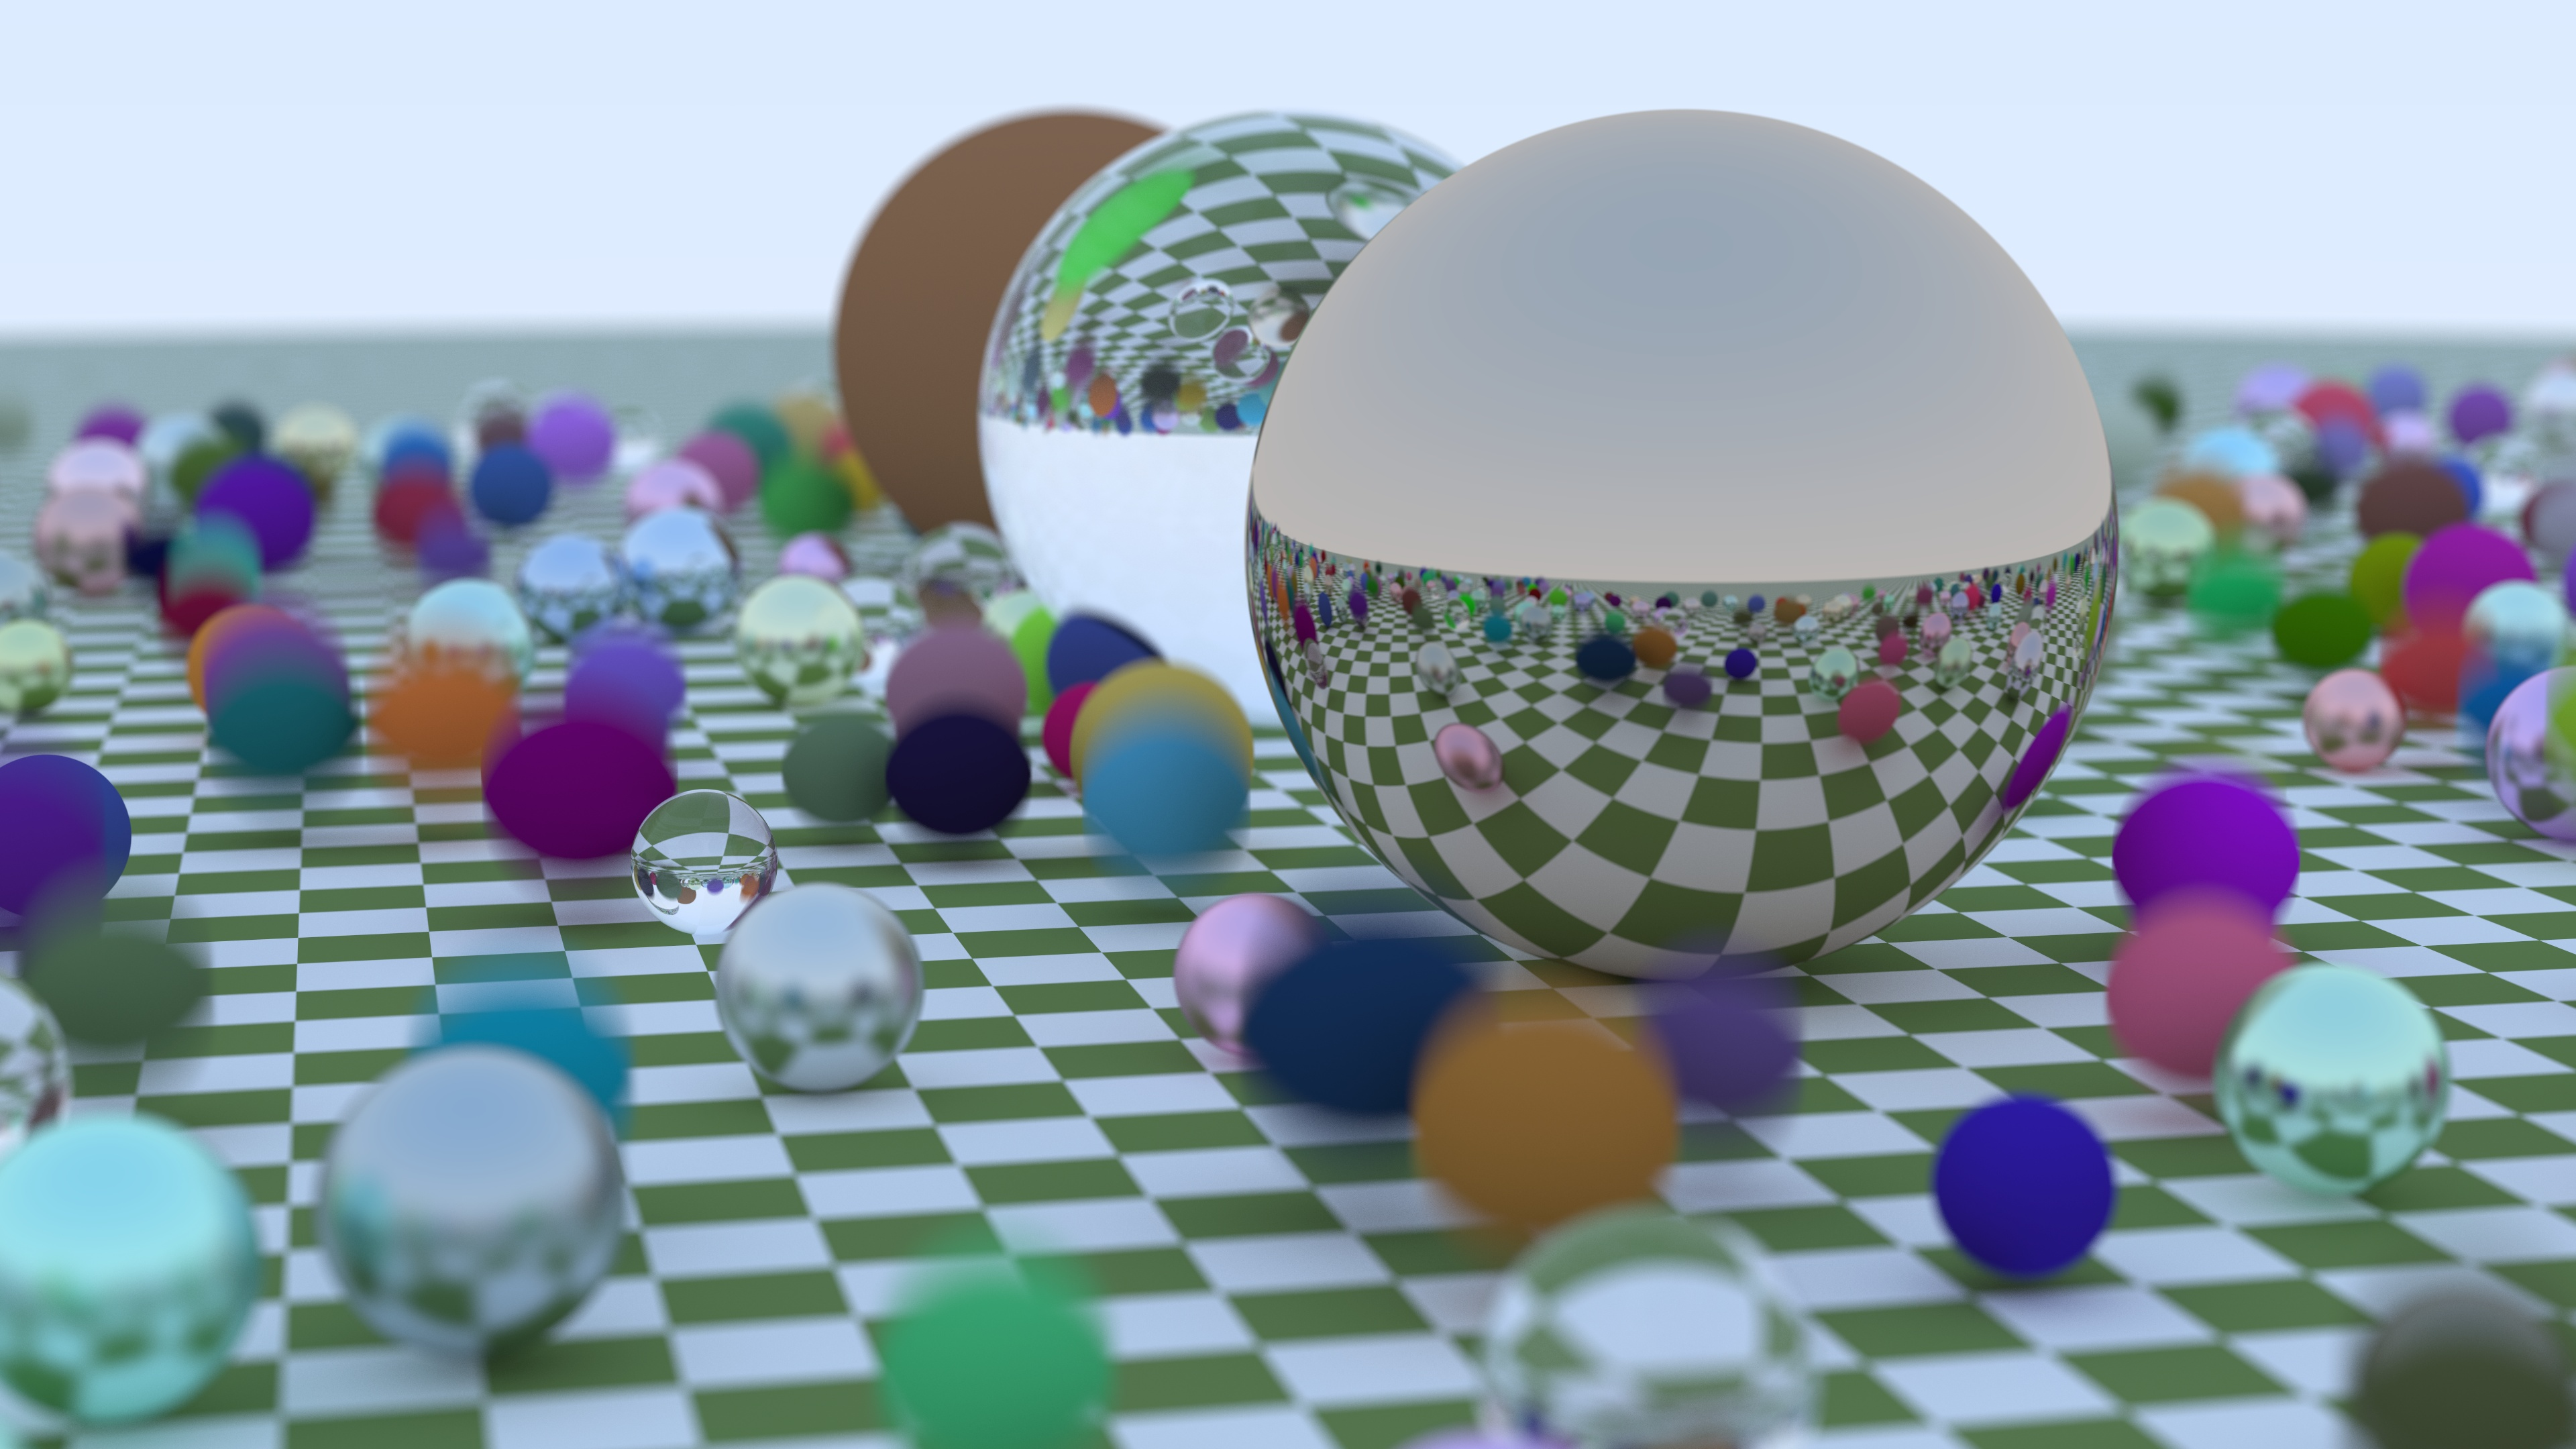
\includegraphics[width=0.7\linewidth]{../_results/motion_blur_checker}
	\caption{Motion Blur Checker}
	\label{fig:motionblurchecker}
\end{figure}
This scene adds a simple procedural texture (checker texture) to the last one.

\subsection{Earth}
\begin{figure}[H]
	\centering
	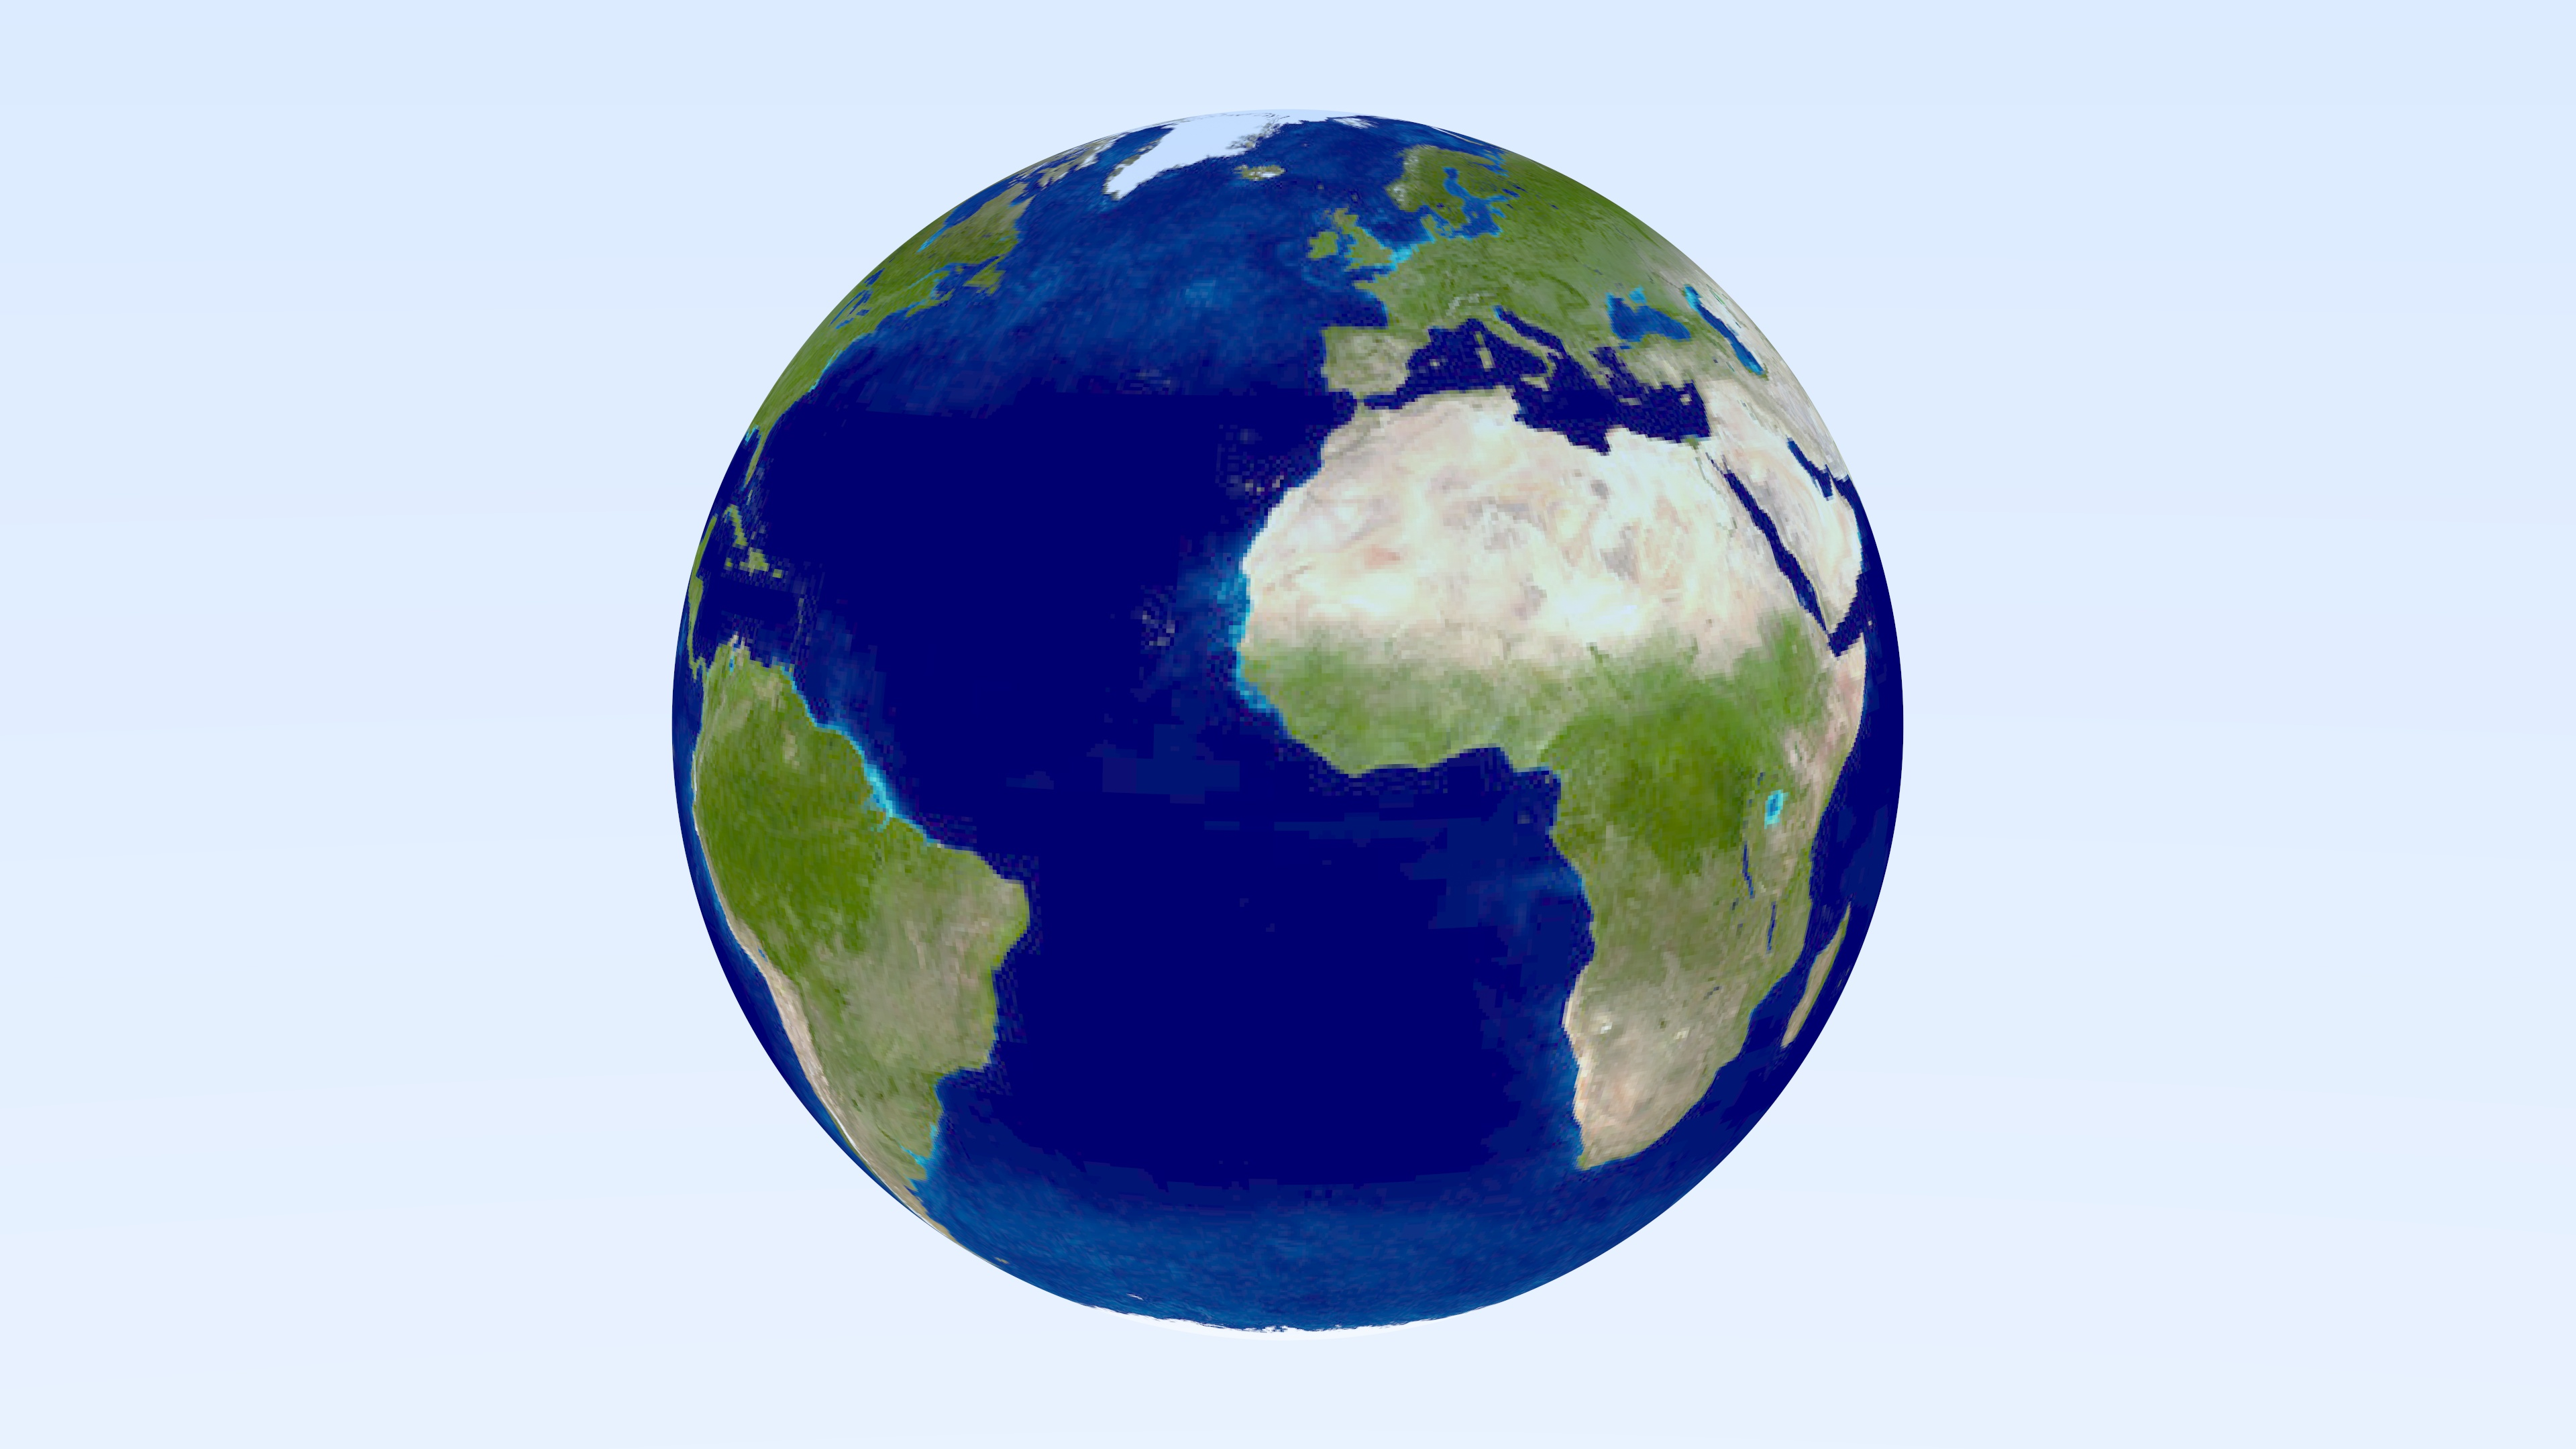
\includegraphics[width=0.7\linewidth]{../_results/earth}
	\caption{Earth}
	\label{fig:earth}
\end{figure}
This scene is a ball with image texture.

\subsection{Cornell Box Series}
\begin{figure}[H]
	\centering
	\includegraphics[width=0.5\linewidth]{../_results/cornell_box_empty}
	\caption{Cornell Box Empty}
	\label{fig:cornellboxempty}
\end{figure}
This is an empty Cornell Box constructed with axis-aligned rectangles.

\begin{figure}[H]
	\centering
	\includegraphics[width=0.5\linewidth]{../_results/cornell_box_two_blocks}
	\caption{Cornell Box Tow Blocks}
	\label{fig:cornellboxtwoblocks}
\end{figure}
\noindent
Added two boxes to the last scene.

\begin{figure}[H]
	\centering
	\includegraphics[width=0.5\linewidth]{../_results/cornell_box}
	\caption{Cornell Box}
	\label{fig:cornellbox}
\end{figure}
\noindent
Add rotation to the two boxes. Color bleeding is obvious on two surfaces facing walls.

\subsection{Cornell Box Participating Media}
\begin{figure}[H]
	\centering
	\includegraphics[width=0.5\linewidth]{../_results/cornell_box_participating_media}
	\caption{Cornell Box Participating Media}
	\label{fig:cornellboxparticipatingmedia}
\end{figure}
This scene replace the two original boxes with participating media boxes. These boxes are assigned with isotropic material to simulate the effect of smoke. This is a technique often used in volumetric rendering. 

\subsection{Book2 Final}
\begin{figure}[H]
	\centering
	\includegraphics[width=0.8\linewidth]{../_results/book_2_final}
	\caption{Book2 Final}
	\label{fig:book2final}
\end{figure}
This scene is a modified version of the one used by Peter Shirley in Ray Tracing Mini-Books 2. It combines may techniques. The whole scene is filled with thin smoke, rendered using participating media. The orange ball on the top left shows motion blur. The earth ball shows image textures. The marble ball in the middle is a complex example of procedural texture computed using Perlin noise. The box on the top right contains 10000 balls as components and use BVH to accelerate.

\subsection{Test Obj}
\begin{figure}[H]
	\centering
	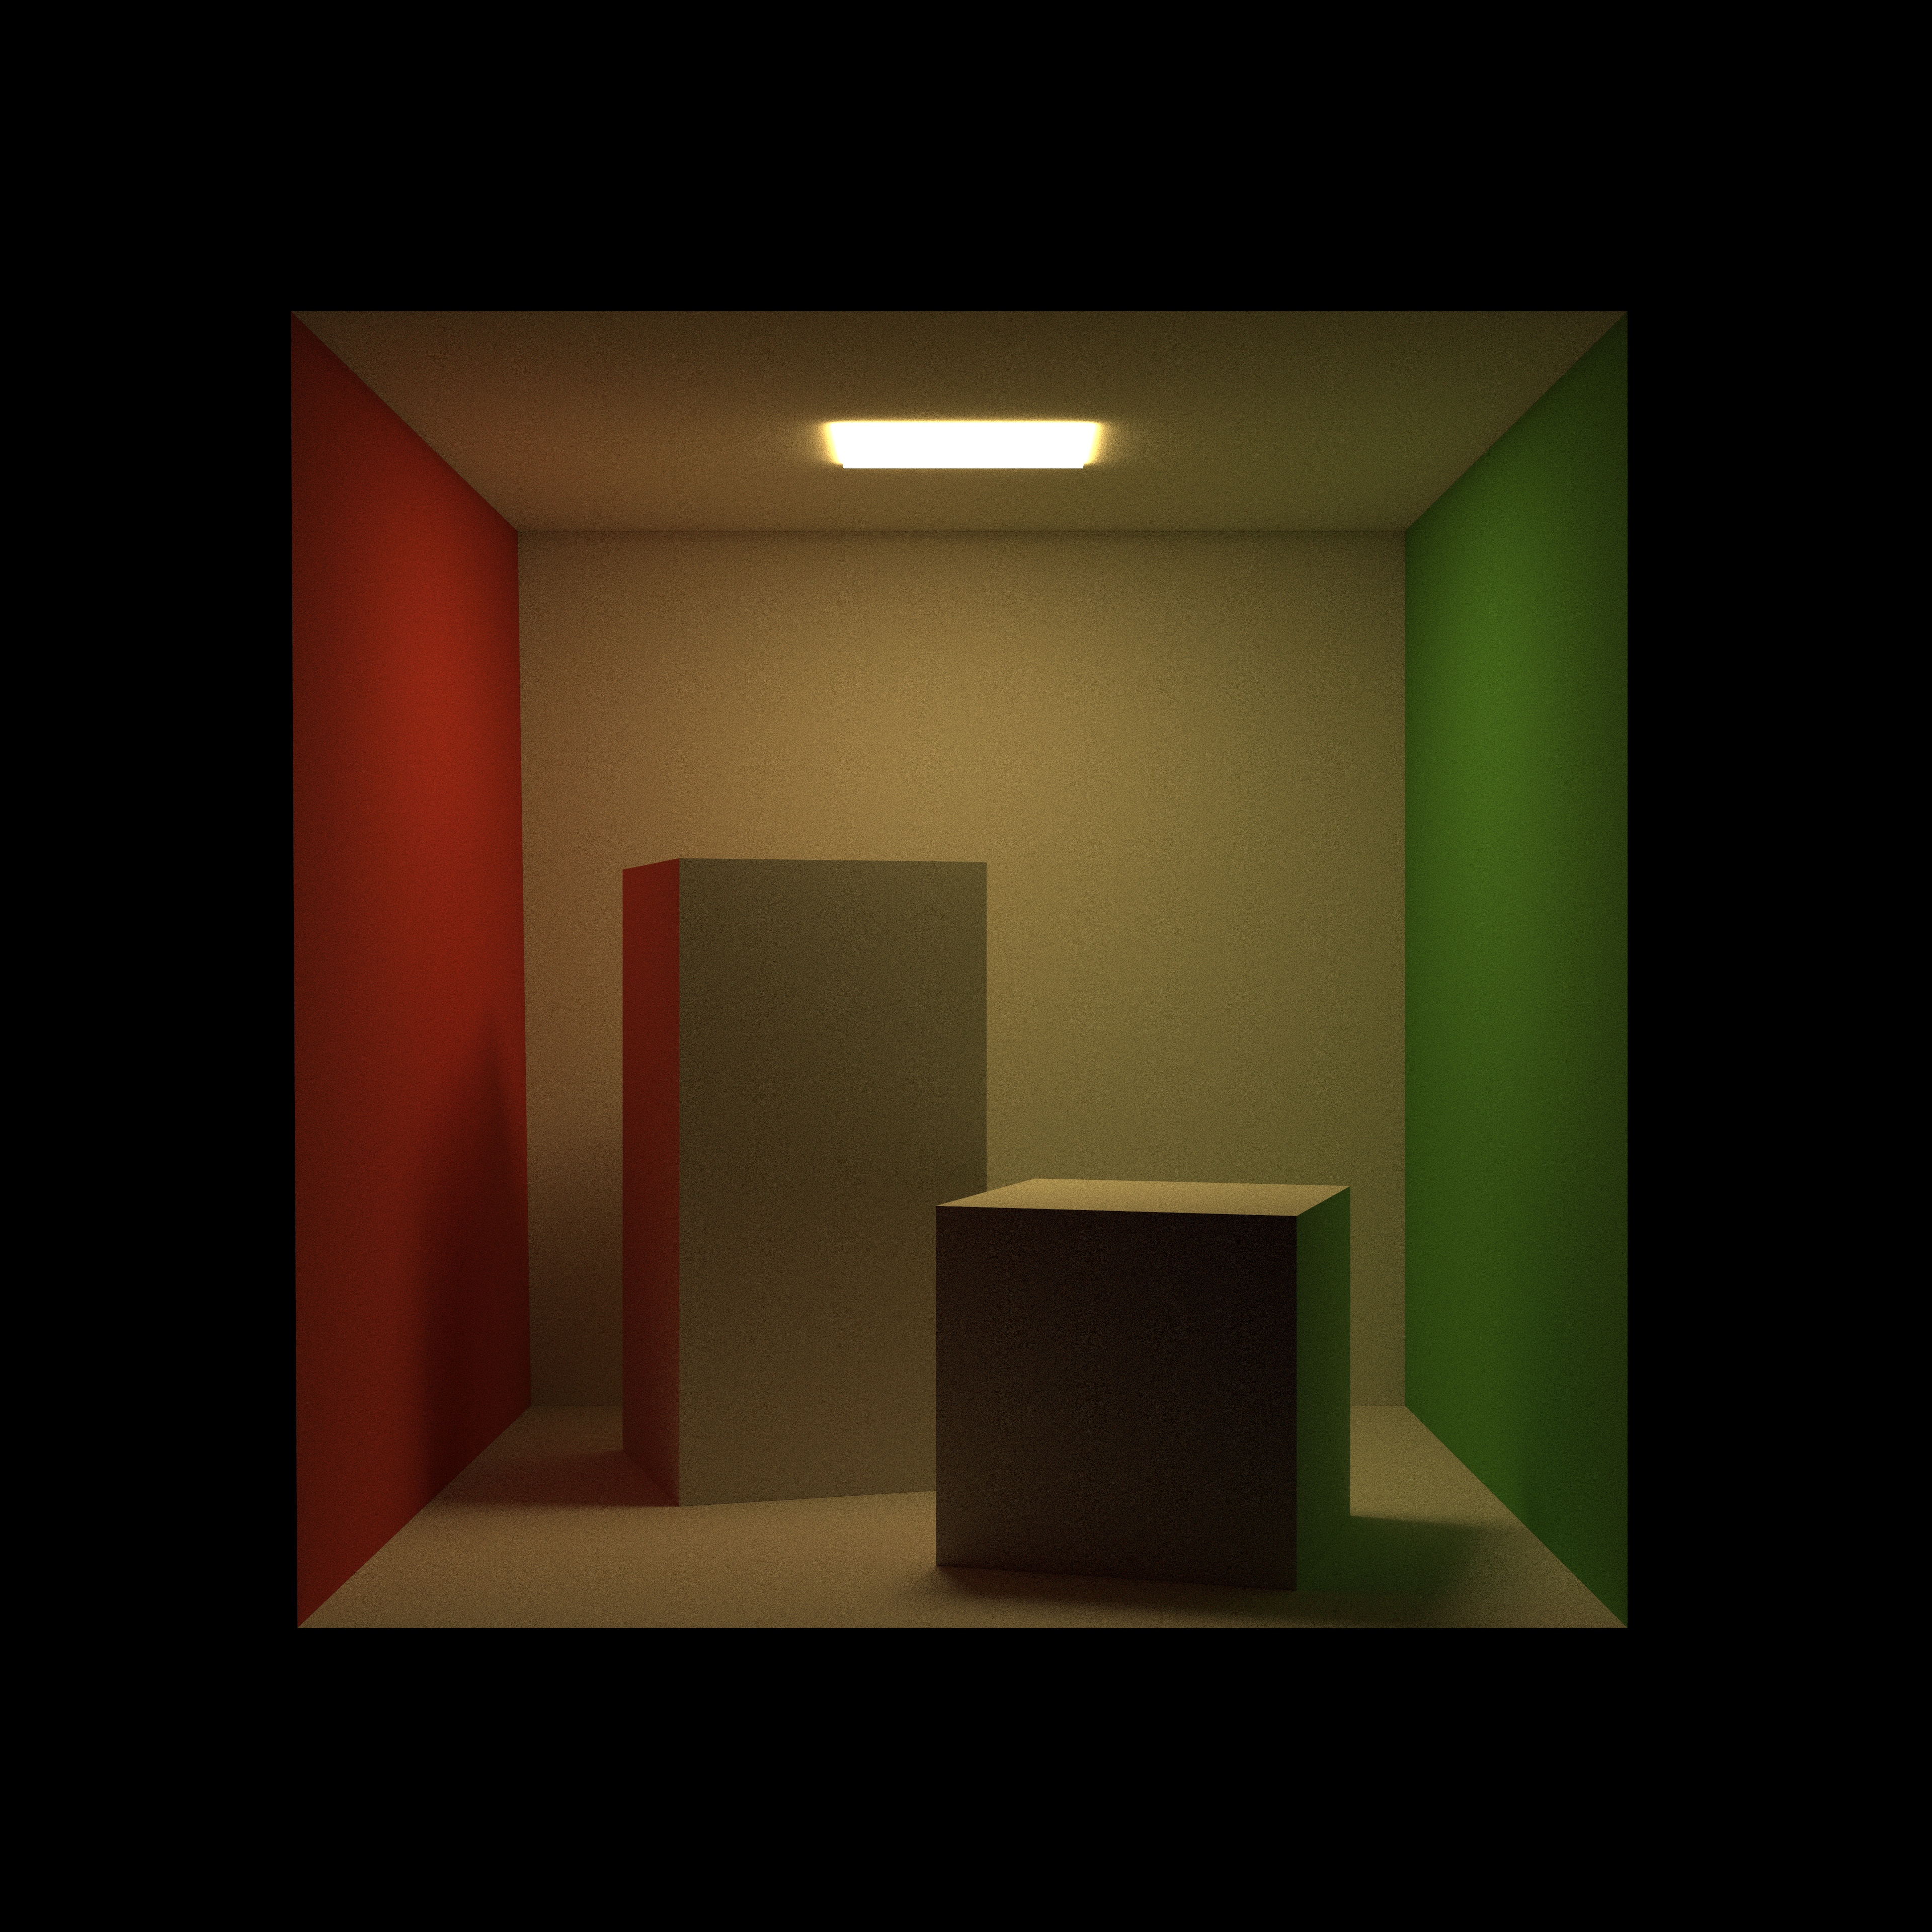
\includegraphics[width=0.45\linewidth]{../_results/test_obj}
	\caption{Test Obj}
	\label{fig:testobj}
\end{figure}
A simple scene used in obj test. This Cornell Box is made of triangles. It is stored in a .obj file (with material description in .mtl file) and imported using Tinyobjloader.

\subsection{Sponza Sun}
\begin{figure}[H]
	\centering
	\includegraphics[width=0.45\linewidth]{../_results/sponza_sun}
	\caption{Sponza Sun}
	\label{fig:sponzasun}
\end{figure}
This scene is a more complicated one with image textures. Note that in this scene, a biased sampling technique is used such that the sun gets more samples.

\subsection{Sponza Crytek Series}
\begin{figure}[H]
	\centering
	\includegraphics[width=0.8\linewidth]{../_results/sponza_crytek_cloudy}
	\caption{Sponza Crytek Cloudy}
	\label{fig:sponzacrytekcloudy}
\end{figure}
This scene is a remastered version of the last one from Crytek cooperation. It is rendered unbiasedly with Path Tracing. Note that bump map is enabled to add more details to the geometry (like the lion in the back). The following one is the same scene with a more complicated skybox. It can be used to simulate extremely sunny weather.

\begin{figure}[H]
	\centering
	\includegraphics[width=0.8\linewidth]{../_results/sponza_crytek_sunny}
	\caption{Sponza Crytek Sunny}
	\label{fig:sponzacryteksunny}
\end{figure}


\subsection{Photon Mapping Series}
A bunny rendered using Photon Mapping. When rendering the first image, photon tracing depth is set to one so that the caustic effect can be seen clearly. The correct effect is shown in the second image.

\begin{figure}[H]
	\centering
	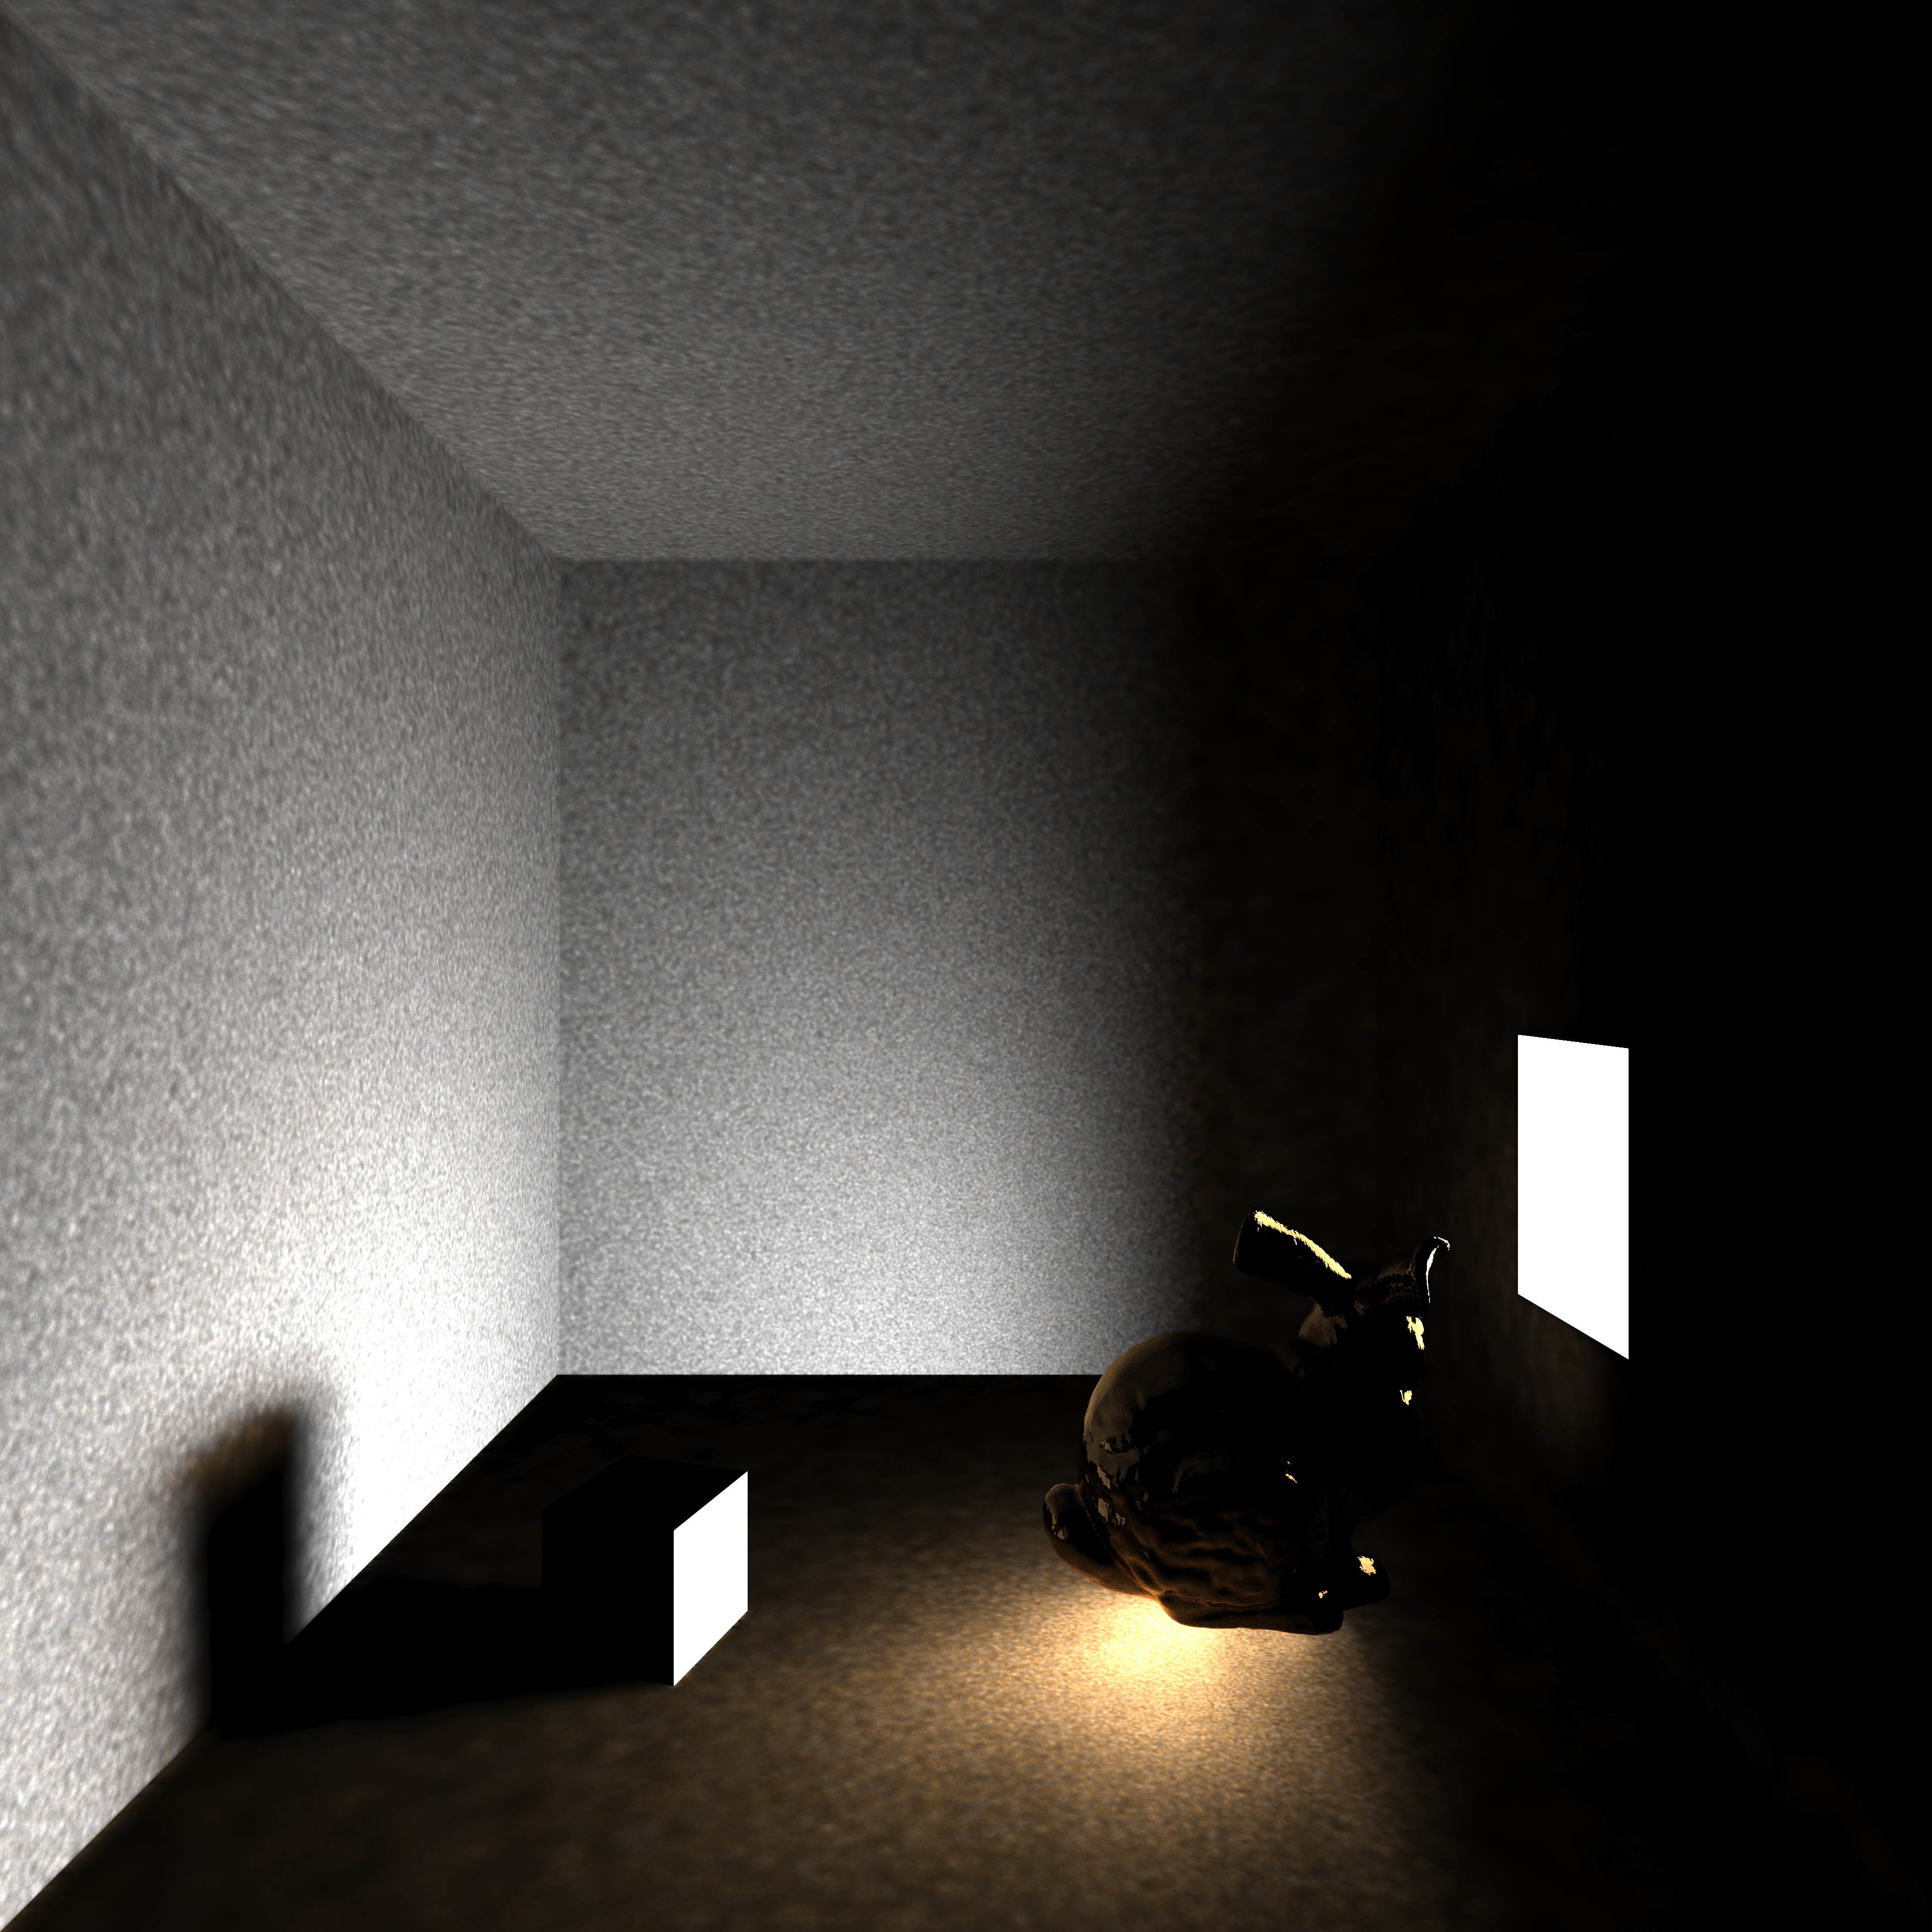
\includegraphics[width=0.5\linewidth]{../_results/photon_mapping_bunny_caustic}
	\caption{Photon Mapping Bunny Caustic}
	\label{fig:photonmappingbunnycaustic}
\end{figure}

\begin{figure}[H]
	\centering
	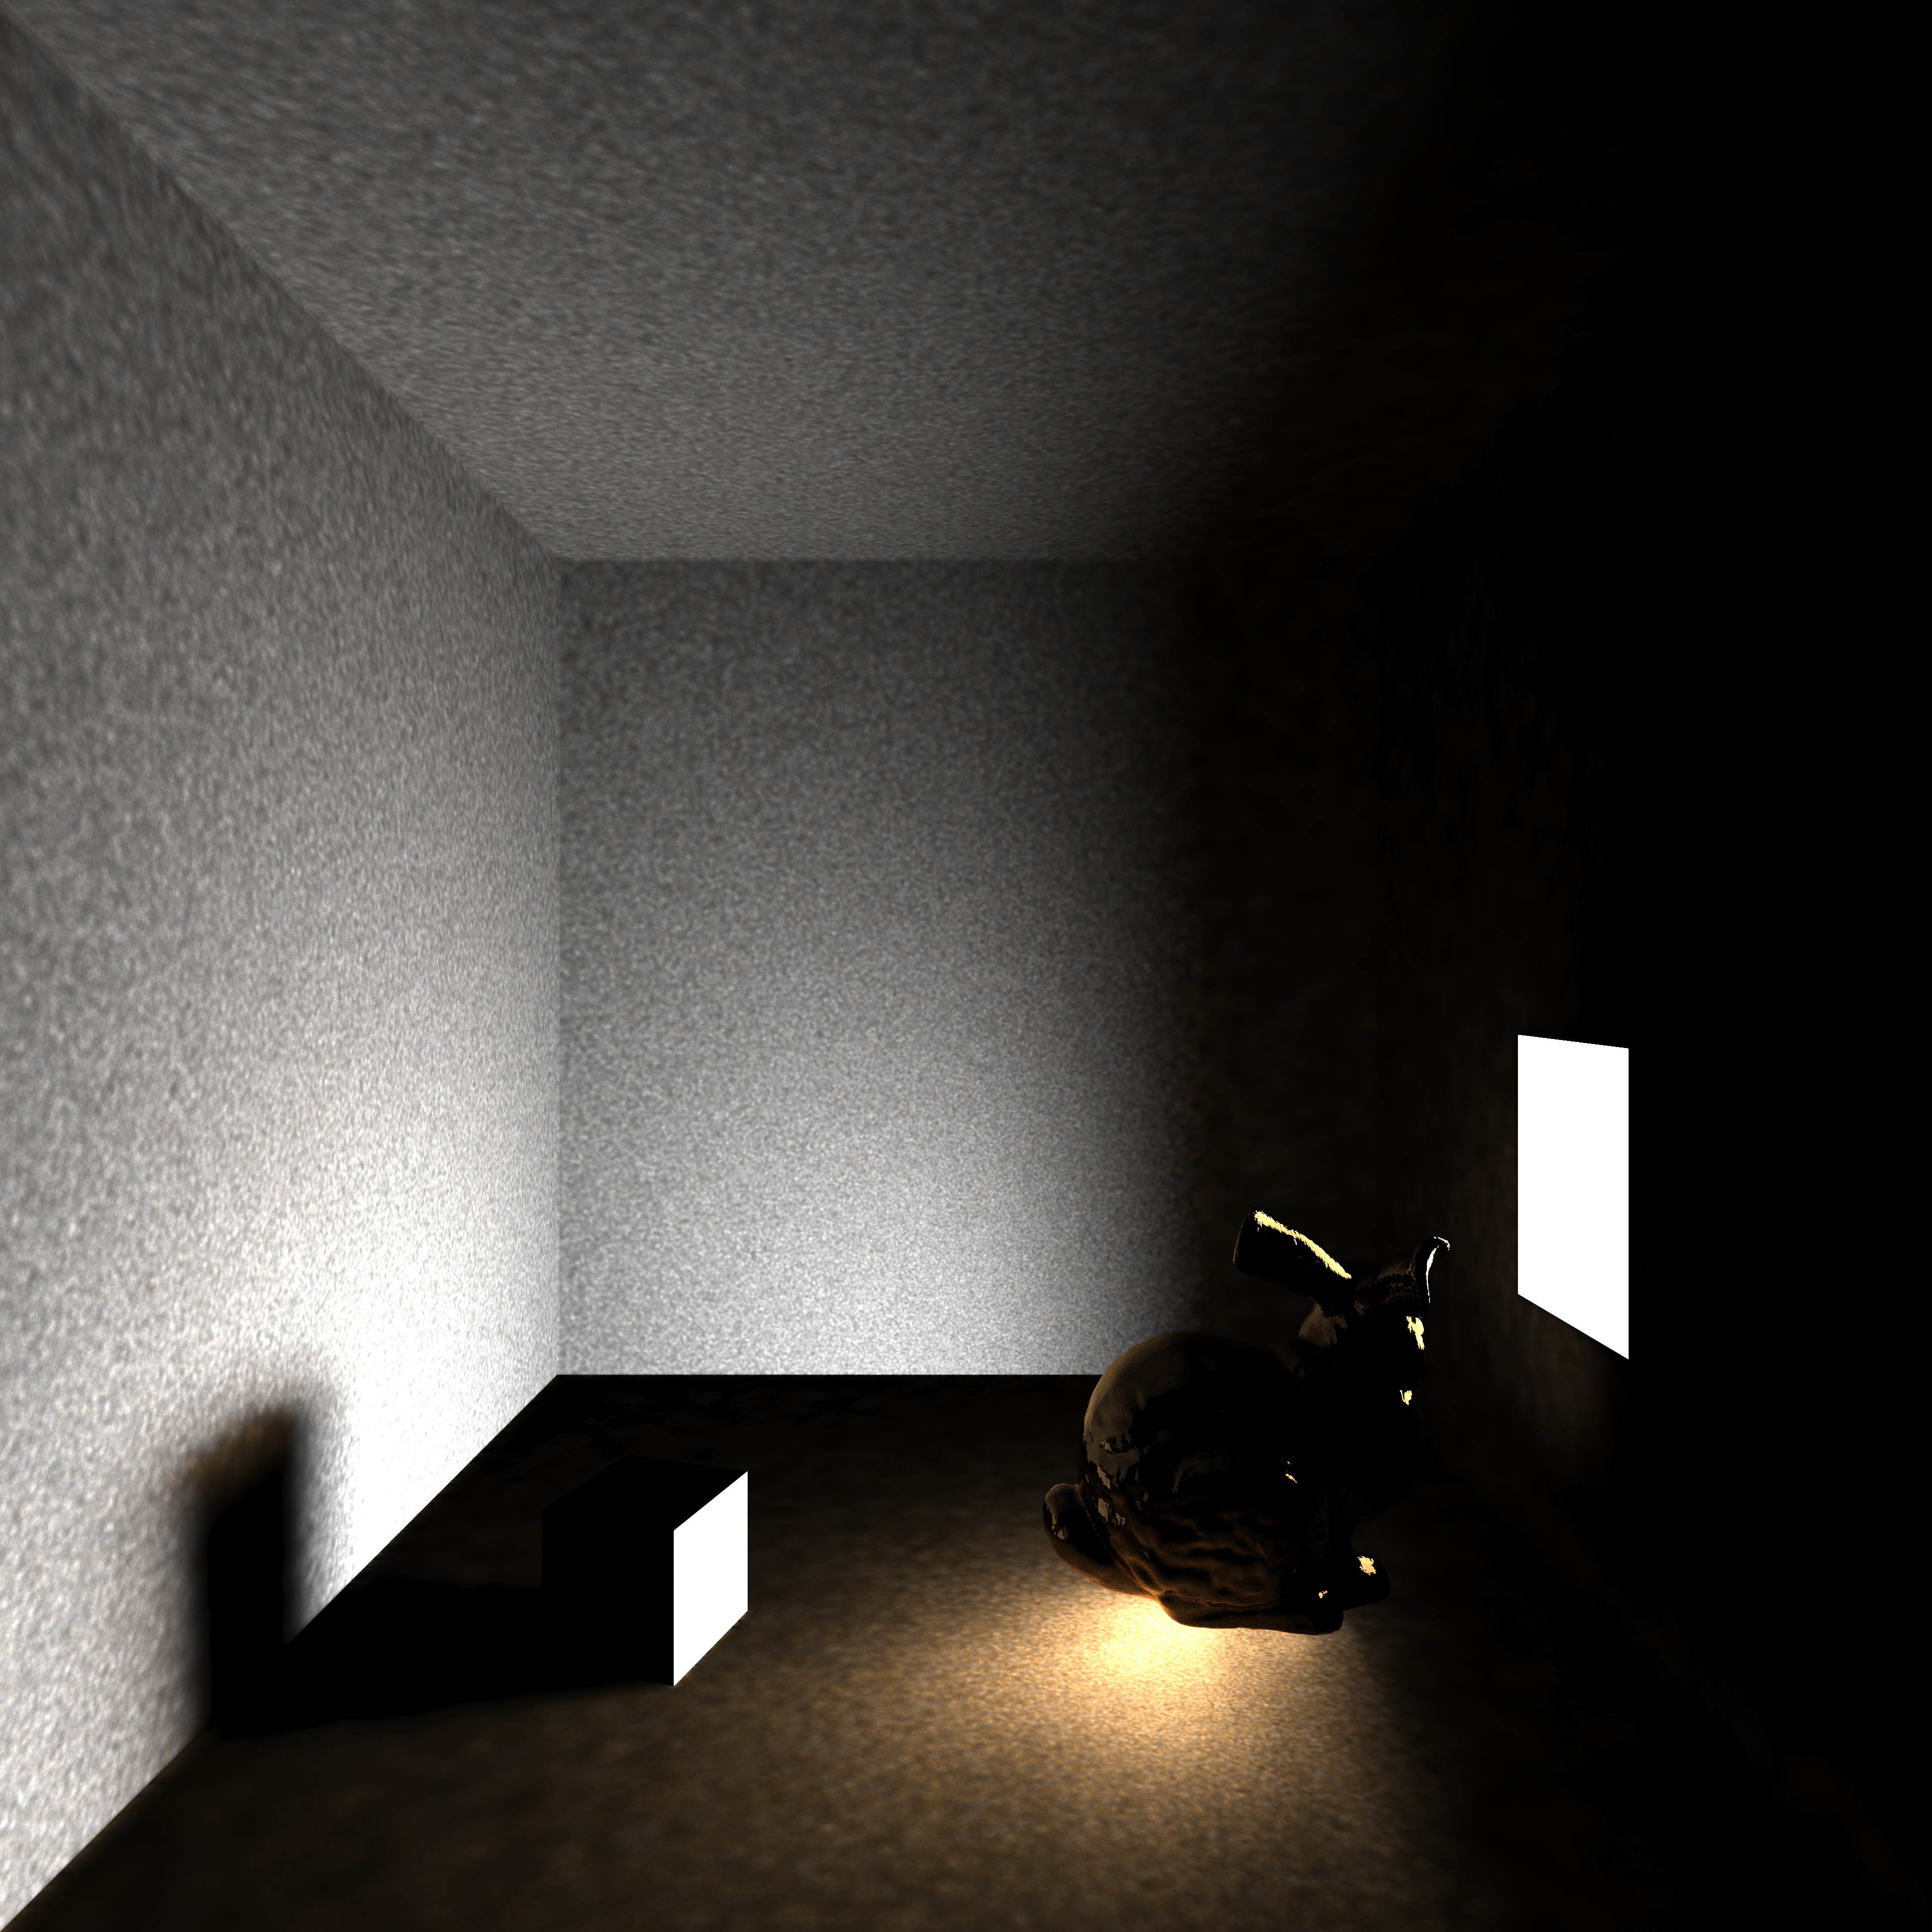
\includegraphics[width=0.5\linewidth]{../_results/photon_mapping_bunny}
	\caption{Photon Mapping Bunny}
	\label{fig:photonmappingbunny}
\end{figure}

\newpage
\section{Usage}

\large \textbf{How set scene before compilation}

\normalsize
\noindent
\textbf{step 1:} set image settings (customization (e.g. changing aspect$\_$ratio to 16.0 / 9.0) can be done by modifying render$\_$scene in main.cpp)

\noindent
\textbf{step 2:} choose integrator (Photon Mapping only supports one scene, Path Tracing has step 3 of setting scene)

\noindent
\textbf{step 3:} set scene, camera and skybox (scene functions can be found in src/scenes) \\

\noindent
\large \textbf{How to run this renderer}

\normalsize
\noindent
\textbf{Windows:}

\noindent
\textbf{step 1:} compile with CLion using MSVC compiler

\noindent
\textbf{step 2:} run "Project.exe 8", here 8 means using 8 threads (after running we will get 8 .partial files)

\noindent
\textbf{step 3:} run "packager.exe 8", here 8 means combining 8 partial files (after running we will get a .ppm image, which can be opened using OpenSeeIt)

\noindent
\textbf{step 4:} run python convert.py, which converts .ppm into .jpg (note that opencv for python is required to run this)

\noindent
\textbf{Linux:}

run "bash linux$\_$run.sh", which compiles the renderer, uses 80 processes to run it and process result into a .ppm and a .jpg file. (Note that for default Sponza Crytek scene, about 150 GB memory is required. This requirement is proportional to the number of processes.)








\section{Renderer Structure}
The basic structure of this renderer is as follows:

\subsection{Basic Renderer:}
\noindent
\textbf{Integrator: } Monte Carlo Path Tracing, Photon Mapping.

\noindent
\textbf{Accelerator: } BVH (AABB with SAH), Kd-Tree.

\noindent
\textbf{Hardware Acceleration: } OpenMP on Windows, Multi-processing on Linux.

\subsection{Objects: }
\noindent
\textbf{Hittable Objects: } Triangle, Triangular Mesh, Box, Sphere.

\noindent
\textbf{Complex Models: } .obj Model with .mtl Material Description.

\noindent
\textbf{Skybox: } Constant Skybox, Directional Skybox, Realistic Skybox, Multi-layer Skybox.

\noindent
\textbf{Transforms: } Rotation, Translation.

\subsection{Materials \& Textures}
\noindent
\textbf{Materials: } Lambertian, Metal, Dielectric, PBR material, Isotropic, Diffuse Light.

\noindent
\textbf{Textures: } Color Texture, Checker Texture, Perlin Noise Texture, Marble Texture, Image Texture, Bump Texture.

\subsection{Visual Effects}
\noindent
\textbf{Camera Effects: } Off-focus Blur, Motion Blur.

\noindent
\textbf{Volumetric Rendering: } Participating Media.

\noindent
\textbf{Other Visual Effects: } Gamma Correction, Caustic.

\section{Code Explanation}

\section{References}
\noindent
\textbf{Code References: }

\noindent
\textbf{[1]} Ray Tracing Mini-books, by Peter Shirley (https://raytracing.github.io)

\noindent
\textbf{[2]} Physically Based Rendering: From Theory to Implementation, by Matt Pharr, Wenzel Jakob, and Greg Humphreys (https://github.com/mmp/pbrt-v3)

\noindent
\textbf{[3]} Dezeming Family (https://dezeming.top/)

\noindent
\textbf{External Libraries: }

\noindent
\textbf{[1]} Tinyobjloader (https://github.com/tinyobjloader/tinyobjloader)

\noindent
\textbf{[2]} stb$\_$image (https://github.com/nothings/stb)

\noindent
\textbf{Model Resources: }

\noindent
\textbf{[1]} Morgan McGuire, Computer Graphics Archive, July 2017 (https://casual-effects.com/data)

\end{document}